\iffalse
\documentclass[epj,nopacs,fleqn]{svjour}
\smartqed
\usepackage[T1]{fontenc}
\usepackage[utf8]{inputenc}
\usepackage{cite,epsfig,amsmath,graphicx,amssymb,listings,slashed}
\usepackage[colorlinks,citecolor=blue,urlcolor=blue,linkcolor=blue]{hyperref}
\journalname{Eur. Phys. J. C}

\title{MadDM 3.0 EW}
\author{
  Federico Ambrogi\inst{1},
}
\institute{
University of Vienna, Faculty of Physics, Bolzmanngasse 5, A-1090 Wien, Austria \\
email: {\color{blue}federico.ambrogi88@gmail.com}
}

\date{Received: date / Accepted: date}
\titlerunning{MadDM 3.0 EW}
\authorrunning{F.~Ambrogi \textit{et al.}}



\fi

\documentclass[a4paper,11pt]{article}
%\pdfoutput=1 % if your are submitting a pdflatex (i.e. if you have
             % images in pdf, png or jpg format)
\usepackage{jheppub} % for details on the use of the package, please
                     % see the JHEP-author-manual
\usepackage[T1]{fontenc} % if needed
\usepackage{booktabs}

\usepackage{slashed}
%\usepackage{subfigure}
\usepackage{xspace}
\usepackage{booktabs}
%% %simple case: 2 authors, same institution
%% \author{A. Uthor}
%% \author{and A. Nother Author}
%% \affiliation{Institution,\\Address, Country}

\begin{document}
\title{\boldmath MadDM 3.0 EW}

\author[a]{Federico Ambrogi}
\affiliation[a]{University of Vienna, Faculty of Physics, Bolzmanngasse 5, A-1090 Wien, Austria}
% e-mail addresses: one for each author, in the same order as the authors\emailAdd{federico.ambrogi@oeaw.ac.at}
\emailAdd{federico.ambrogi88@gmail.com}

\maketitle




\newcommand{\PPPC}{\texttt{PPPC4DMID}}
\newcommand{\PPPCew}{\texttt{PPPC4DMID\_ew}}
\newcommand{\MG}{\texttt{MadGraph5\_aMC@NLO}}


\newcommand{\run}{\texttt{run\_card.dat}}
\newcommand{\param}{\texttt{param\_card.dat}}
\newcommand{\mchi}{$m_{\chi _D}$}
\newcommand{\maddm}{\texttt{MadDM 3.0}}

\section*{Abstract}
This documents summarises the status of the studies of the discrepancies found in the energy spectra provided in the PPPC4DMID tables (labelled \textbf{PPPC4DMIDew} in MadDM v.3.0) and the spectra produced with MadDM 3.0.



\section{Introduction}
All the information, including the model used and the input cards (\run~ ,\param) can be found at:
\\
{\color{blue} \url{ https://github.com/fambrogi/MadDM} }

\clearpage
\section{PPPC Electroweak Corrections}
In this section the energy spectra for the Cosmic Rays $CRs = e^+, \nu_e , \gamma$ extracted from the \PPPC~and \PPPCew~ Tables are compared, to get an idea of the effect of the EW correction (according the \PPPC collaboration). 

\begin{figure}[!]
\begin{center}
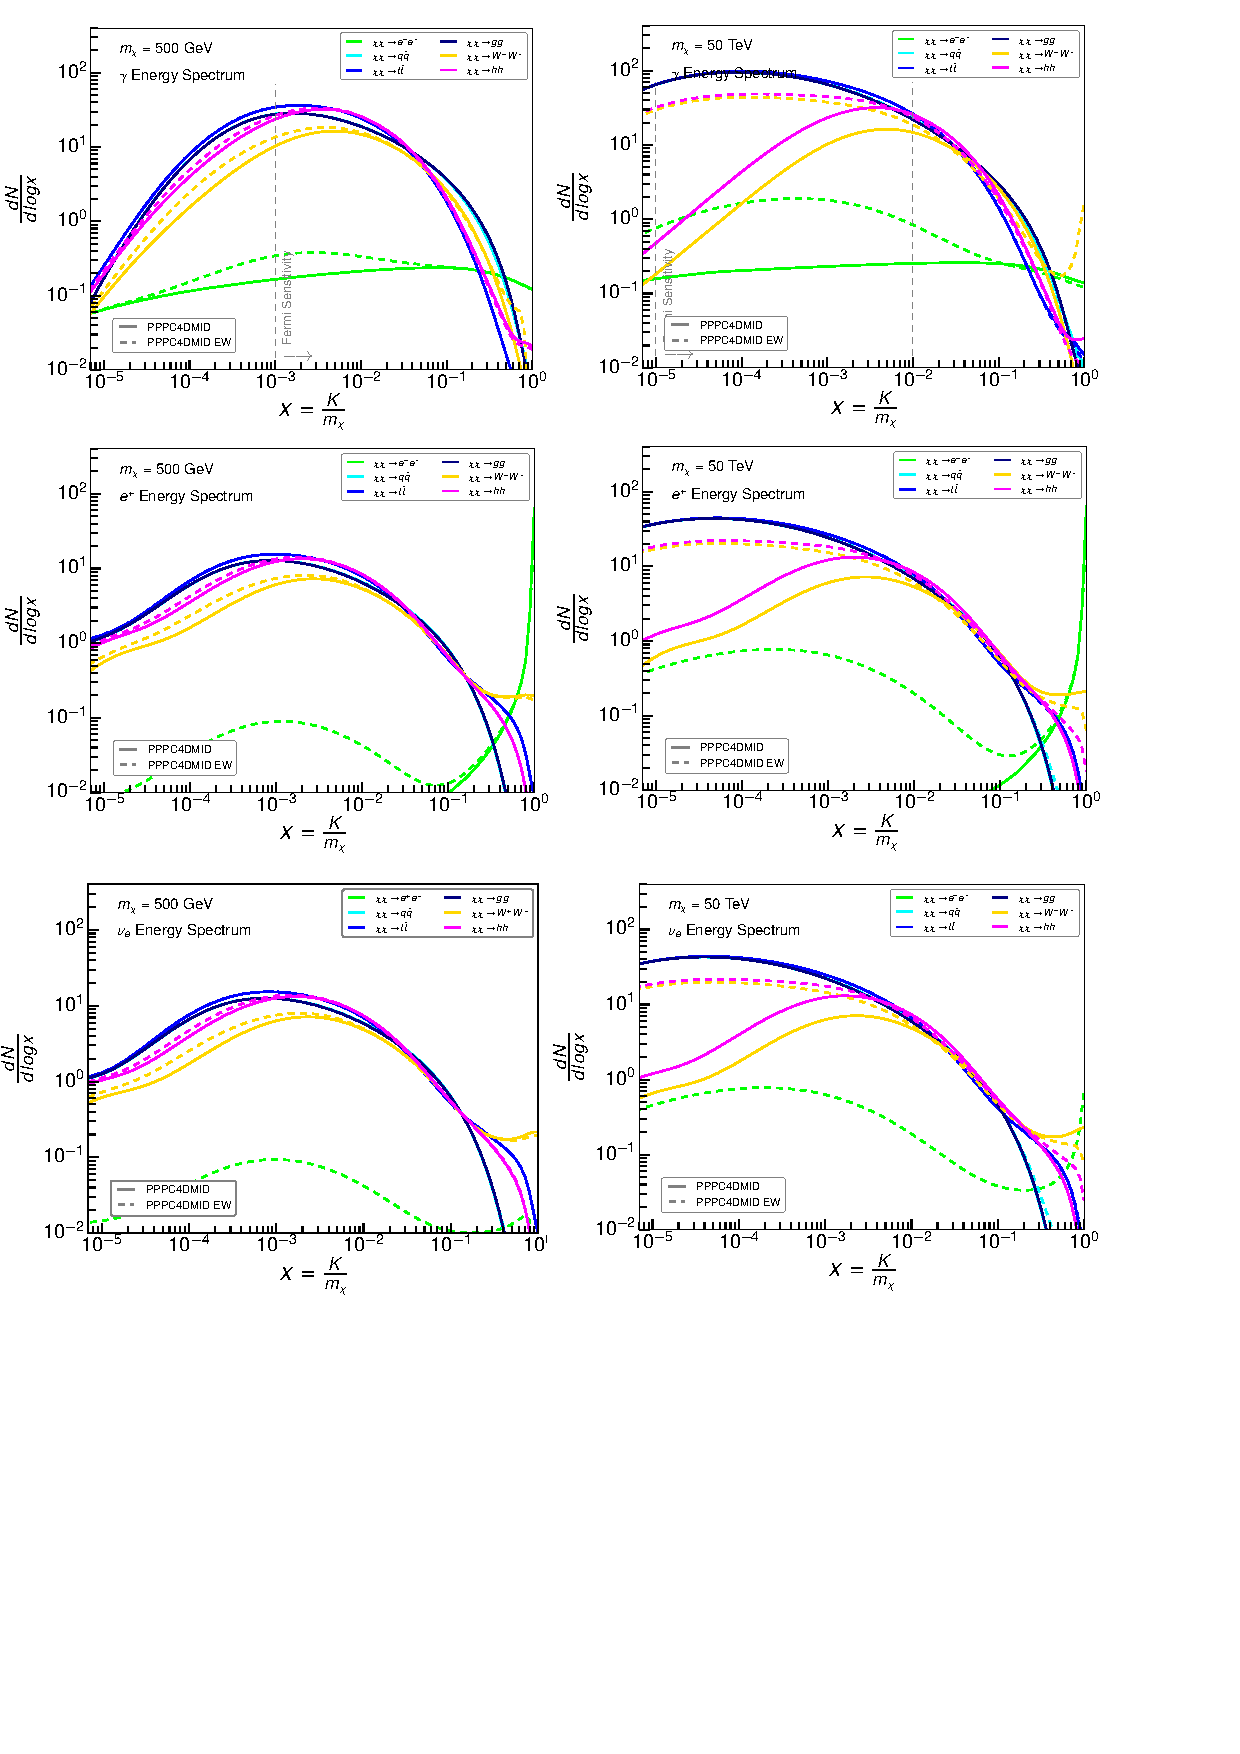
\includegraphics[width=1\textwidth]{Fig/EW_noEW_PPPC.pdf}
\end{center}
\caption{Energy spectra ($\gamma, e^+, \nu _e$) for $m_{\chi}=$500 GeV (left) and 50 TeV (right) extracted from the \PPPC~and \PPPCew~tables, for selected annihilation channels.}
\end{figure}


\clearpage
\section{EW with \MG}
\subsection{Processes}
The processes used for the production of the samples with emission of extra electroweak bosons (Higgs, W and Z bosons) are the following:
\begin{verbatim}
import model DMsimp_s_spin0_EW
define X = W- W+ Z h
generate xd xd~ > w- w+
add process xd xd~ > w- w+ X
add process xd xd~ > w- w+ X X
add process xd xd~ > w- w+ X X X
\end{verbatim}
Note that the short notation e.g. "XXW" includes the lower order processes (in this case only the tree level xdxd>WW) and up to one extra "X" boson, and likewise for the higher order processes. \\

Syntax for excluding diagrams with photons:
\begin{verbatim}
import model DMsimp_s_spin0_EW
define X = W- W+ Z h
generate xd xd~ > w- w+ /a
add process xd xd~ > w- w+ X  /a
add process xd xd~ > w- w+ X X  /a
add process xd xd~ > w- w+ X X X  /a
\end{verbatim}
\\

Relevant parameters in the \run~: 
\begin{verbatim}
*** run_card
1001.0     = ebeam1  
10001.0    = ebeam1  
100001.0    = ebeam1 
\end{verbatim}
for  $m_{\chi_D}$=1 , 10, 100 TeV respectively, and the \param~:
\begin{verbatim}
*** param_card
52 1.00000e+03 # MXd 
54 2.00000e+03 # MY0  (= 2 x MXd )   
\end{verbatim}
\\

\subsection{Cross Sections Comparison}
In Tab. \ref{xsec} the cross sections in [pb] obtained with different runs are shown.
\begin{table*}[!h]
\centering
\renewcommand{\arraystretch}{1.2}
\small
\begin{tabular}{ l | c | c | c | c } \toprule \toprule 
$\mathbf{m_{\chi_D}} $ & $\mathbf{\chi _D \chi _D \rightarrow WW} $ & $\mathbf{\chi _D \chi _D \rightarrow WW X} $ & $\mathbf{\chi _D \chi _D \rightarrow WWX X }$ & $\mathbf{\chi _D \chi _D \rightarrow WW X X X}$ \\  \toprule 
    1.0 TeV (Old) & 474 & 130* & 600 & 600 \\  
    1.0 TeV (Old, no $\gamma$) & 474 & 676 & 704 & - \\  
    1.0 TeV (New) & 173 & 215 & 219 & - \\  
    1.0 TeV (New,AUTO) & 147.3 & 148.2 & - & - \\    

    1.0 TeV (Chiara) & 147.3 & 148.2 & 148.2 & - \\    

  
  10.0 TeV (Old)  & 15.1 $\times 10 ^3$ & 30.501 $\times 10 ^3$ & 37.018 $\times 10 ^3$ & - \\ 
  10.0 TeV (Old,no $\gamma$)  & 15.1 $\times 10^3$  & 2.7 $\times 10 ^7$ & 1.5 $\times 10^{10}$ & - \\ 

  10.0 TeV (New)  & 15.1 $\times 10 ^3$ & 30.542 $\times 10 ^3$  & - & - \\    
  100.0 TeV (Old) & 4.7  $\times 10 ^5$  & - & - & - \\  



    \bottomrule \bottomrule
  \end{tabular}
  \caption{Cross sections in [pb]  for various processes extracted from the LHE files. The "New" cross sections were computed with $N_{Events}$=10,000, while the "Old" ones with $N_{Events}$=100,000. Need to verify the value 130*. }
  \label{xsec}
\end{table*}



\clearpage
\subsection{Spectra for $\chi_D \chi_D \rightarrow e^- e^+$}
The following spectra in Fig. \ref{ee} are obtained with:
\begin{verbatim}
import model /home/federico/Desktop/Tools/MadGraph5/MG5_aMC_v2_6_5/mod\
els/DMsimp_s_spin0_leptons
generate xd xd~ > e- e+
add process xd xd~ > e- e+ z
add process xd xd~ > e- ve~ w+
add process xd xd~ > e+ ve w-
\end{verbatim}
in order to test the EW correction produced ba \MG~ on the electron-positron pairs. Chiara modified the models to include direct couplings of the mediator to the leptons.
However it seems that including the additional processes in \MG~ does not affect at all the spectra. Indeed, in the lhe files there are no neutrinos, W or Z bosons (100k events generated). I additionally tested the $n_1 n_1 \rightarrow e^- e^+$ production (i.e. MSSM) to check that the spectra are indeed the same. 
\begin{figure}[!b]
	\centering
	\subfigure
	{ 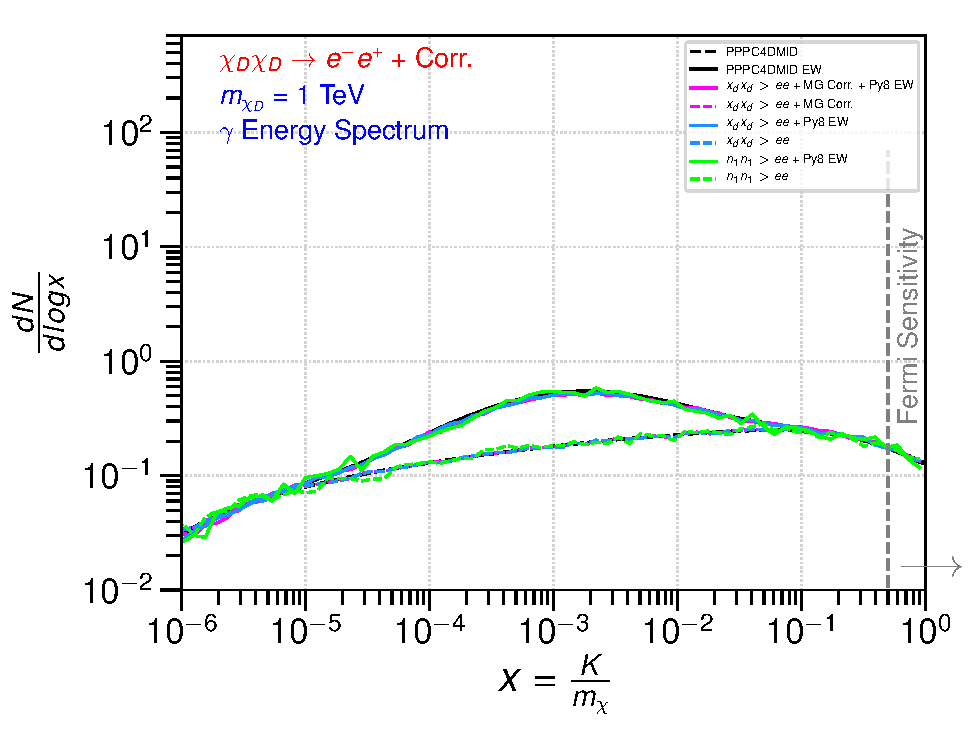
\includegraphics[width=0.49\textwidth]{Fig/xdxd_eeEW/1_gammas_eeEW_1.pdf}}
	\subfigure
	{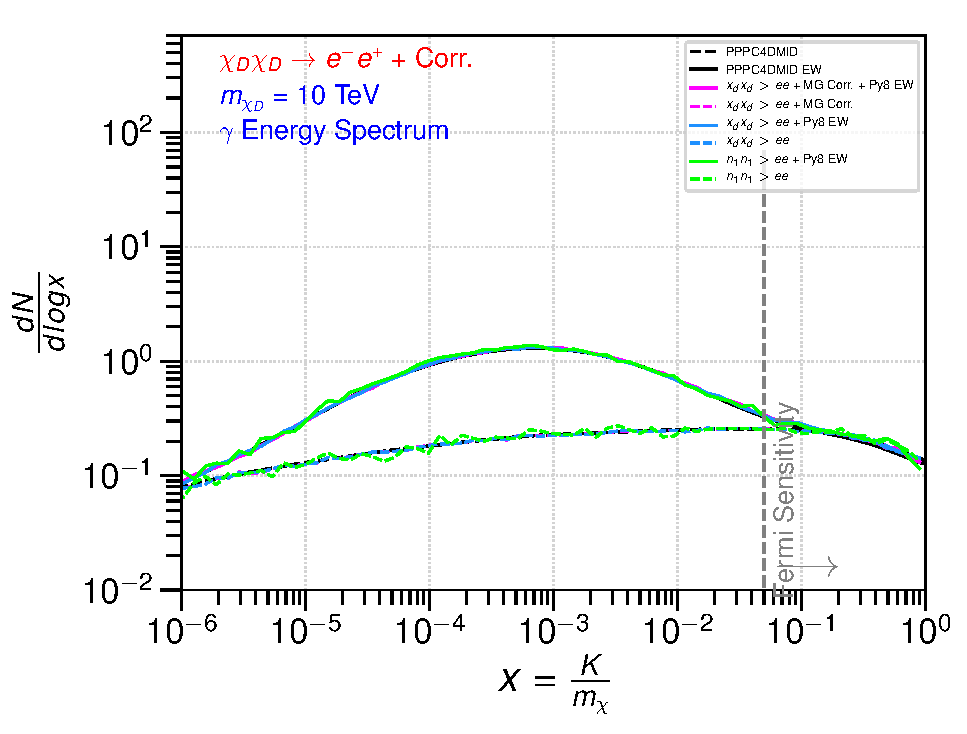
\includegraphics[width=0.49\textwidth]{Fig/xdxd_eeEW/10_gammas_eeEW_10.pdf}}
	\subfigure
	{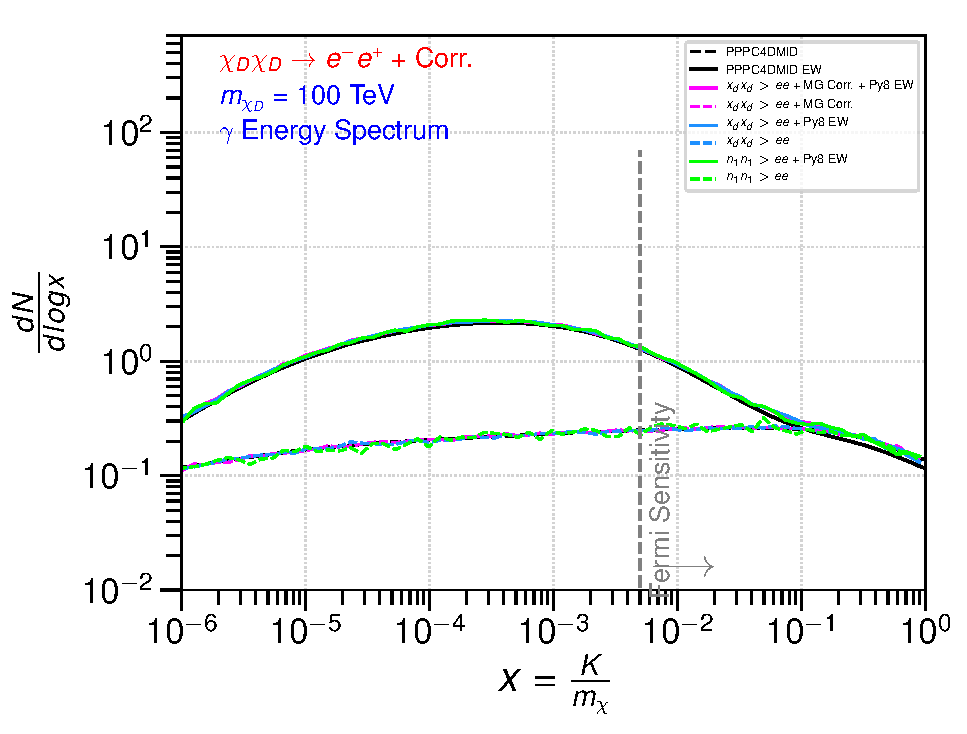
\includegraphics[width=0.49\textwidth]{Fig/xdxd_eeEW/100_gammas_eeEW_100.pdf}}

	\caption{Energy Spectra for the channel $e^- e^p$ using the DM simplified model with couplings to leptons or the MSSM. }
	\label{ee}
\end{figure}
\\
For further test, shown in Fig. \ref{ee_Z}, I generated the samples: 
\begin{verbatim}
import model /home/federico/Desktop/Tools/MadGraph5/MG5_aMC_v2_6_5/mod\
els/DMsimp_s_spin0_leptons
generate xd xd~ > e- e+ z
\end{verbatim}
however \MG~ returns zero events (i.e. cross section equals zero).




\clearpage
\subsection{Spectra for $\chi_D \chi_D \rightarrow WW$}
\subsubsection{$m_{\chi_D}$ = 1 TeV}
\begin{figure}[!b]
\centering
\subfigure
{ 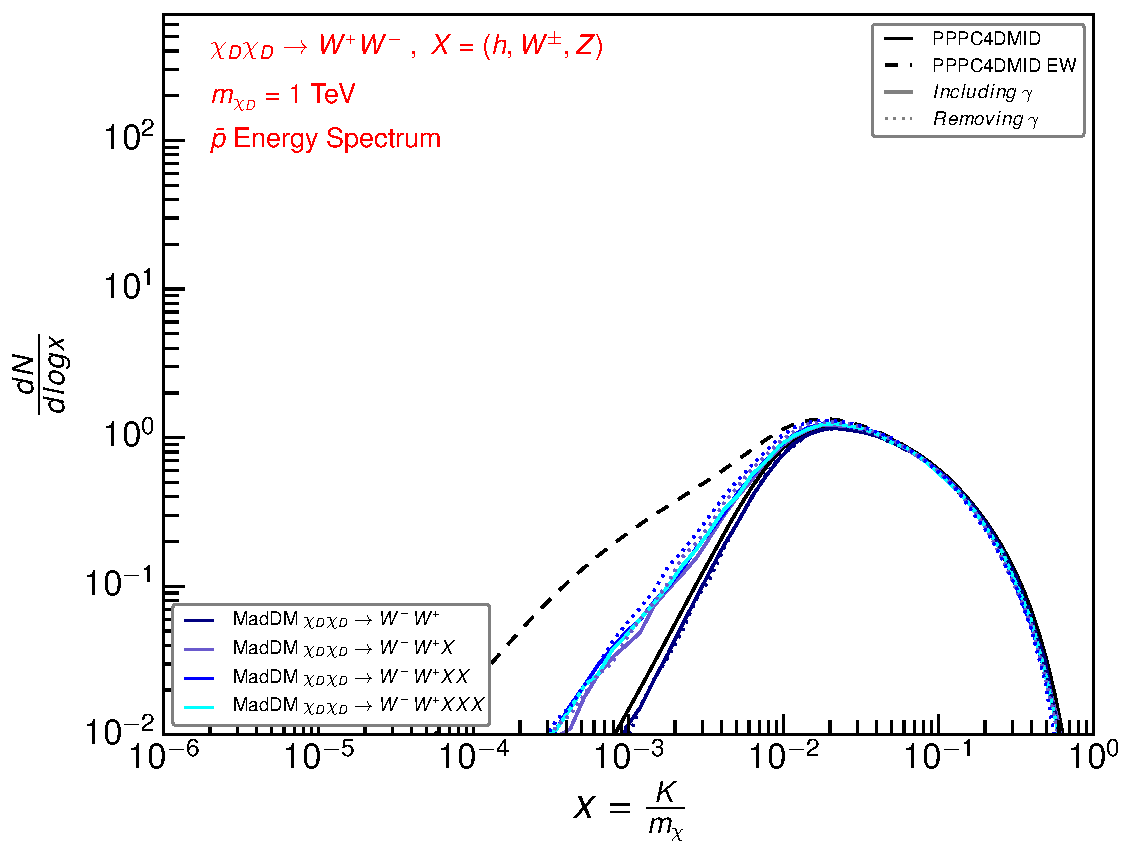
\includegraphics[width=0.49\textwidth]{Fig/1TeV/1_antiprotons_PPPC_Comparison_xdxd_fotone_1.pdf}}
\subfigure
{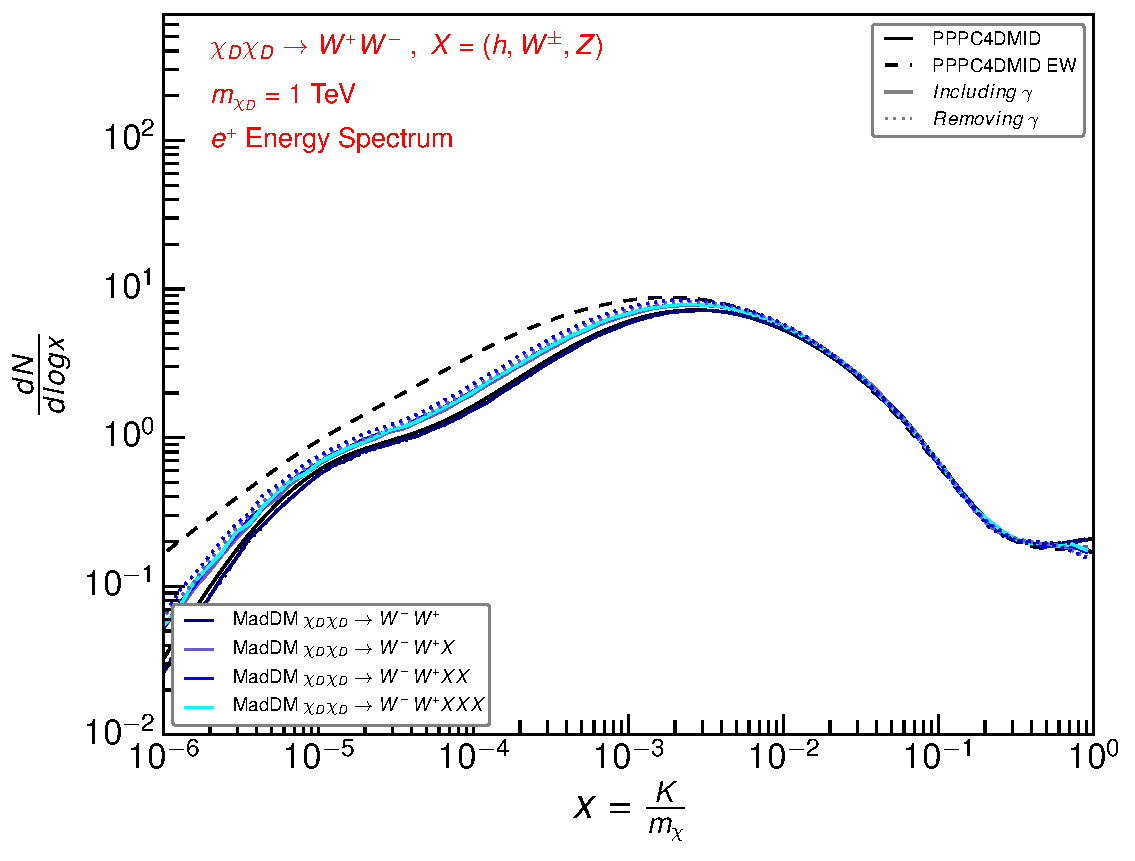
\includegraphics[width=0.49\textwidth]{Fig/1TeV/1_positrons_PPPC_Comparison_xdxd_fotone_1.pdf}}
\subfigure
{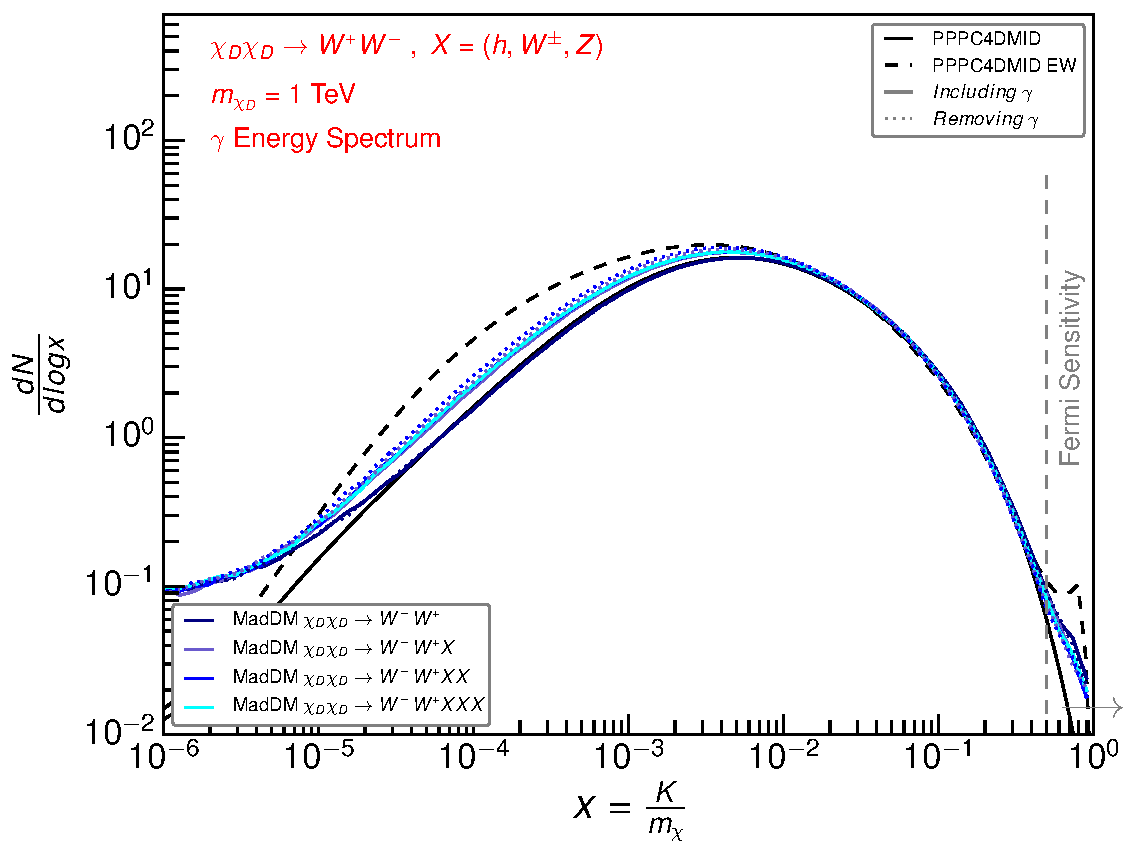
\includegraphics[width=0.49\textwidth]{Fig/1TeV/1_gammas_PPPC_Comparison_xdxd_fotone_1.pdf}}
\subfigure
{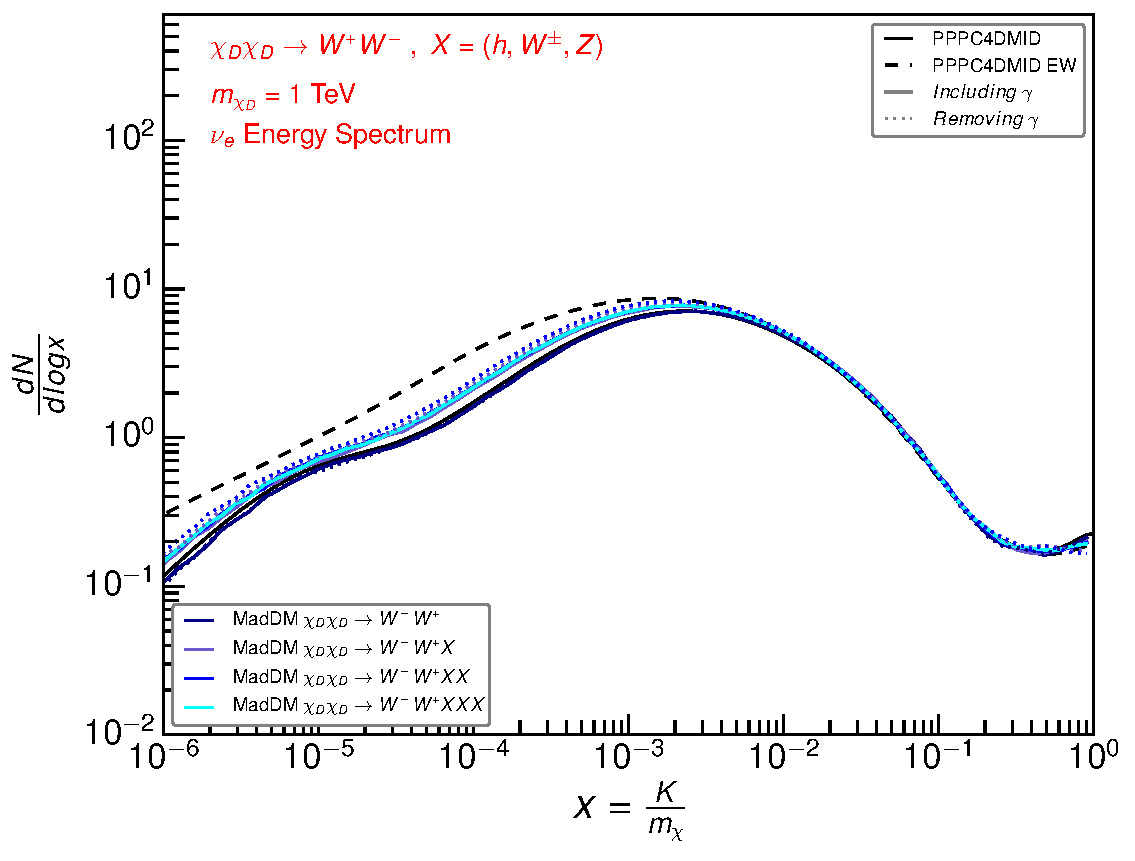
\includegraphics[width=0.49\textwidth]{Fig/1TeV/1_neutrinos_e_PPPC_Comparison_xdxd_fotone_1.pdf}}
\subfigure
{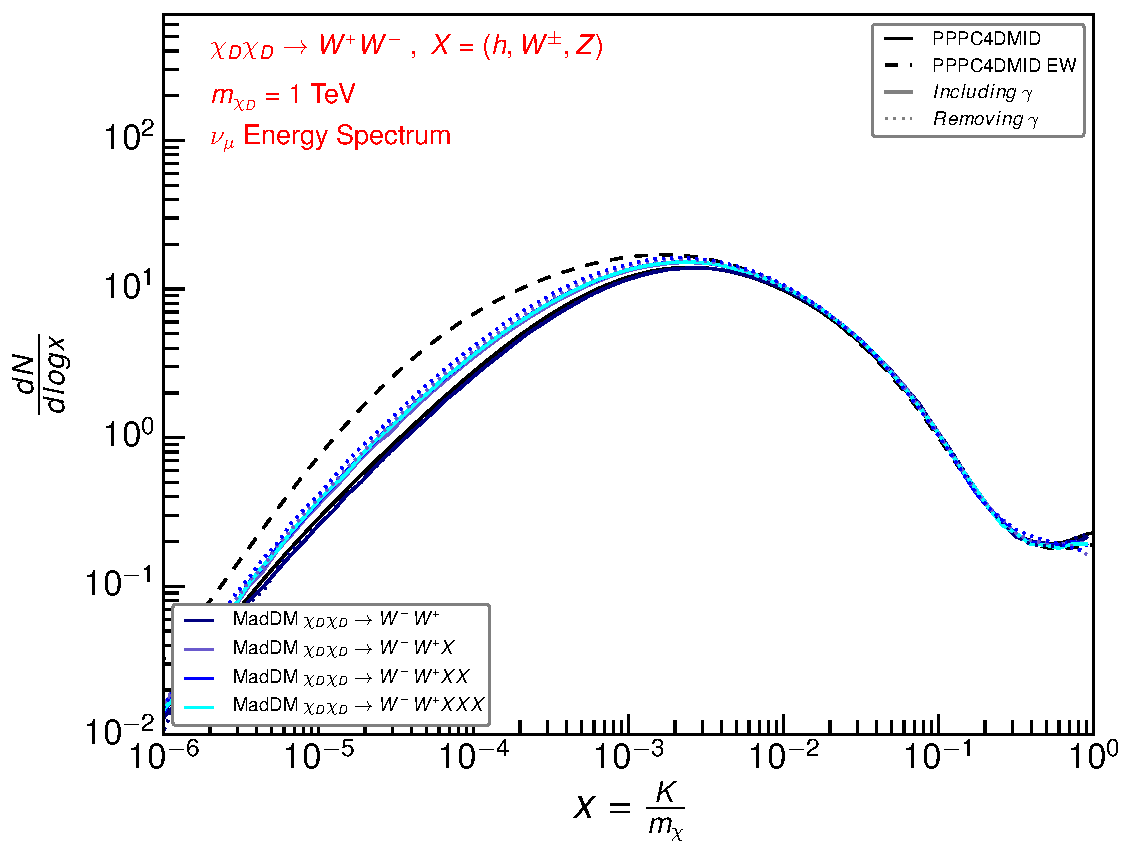
\includegraphics[width=0.49\textwidth]{Fig/1TeV/1_neutrinos_mu_PPPC_Comparison_xdxd_fotone_1.pdf}}
\subfigure
{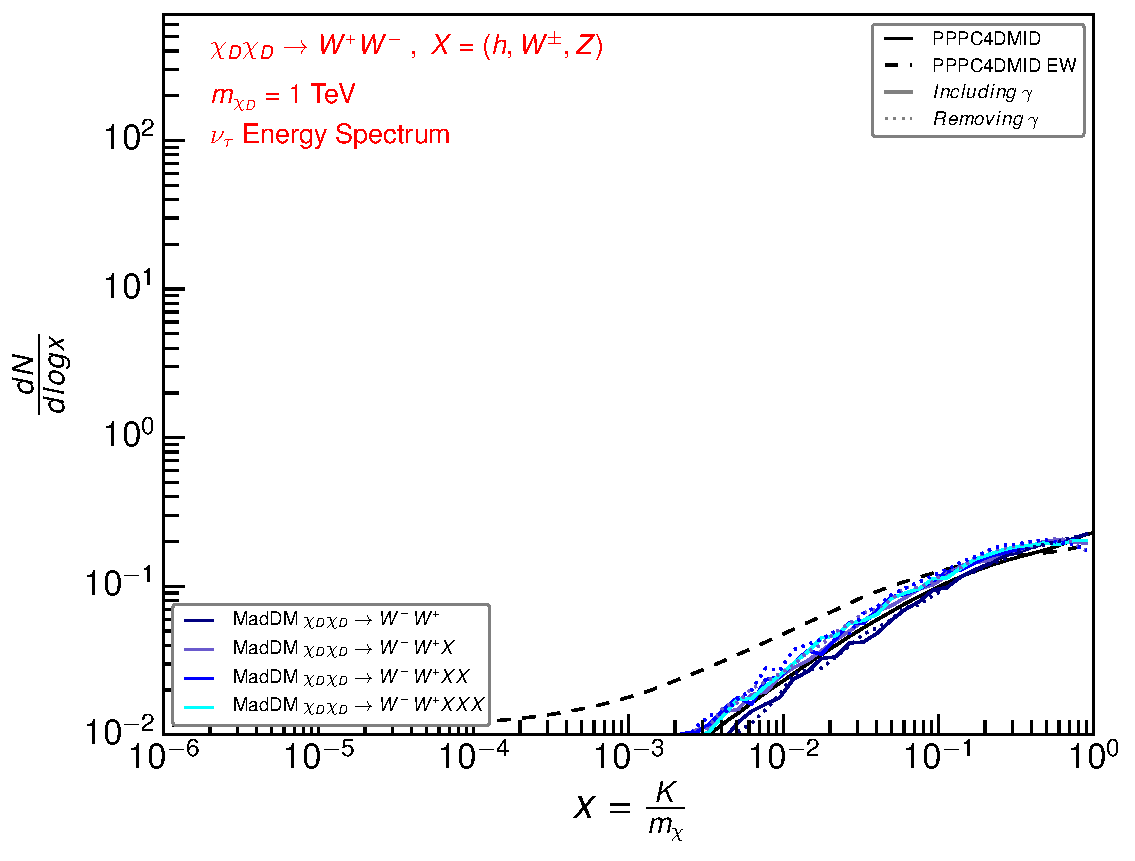
\includegraphics[width=0.49\textwidth]{Fig/1TeV/1_neutrinos_tau_PPPC_Comparison_xdxd_fotone_1.pdf}}
\caption{Energy Spectra for $m_{\chi_D}$ = 1 TeV}
\end{figure}
%
%
%
\clearpage
\subsubsection{"Old" $m_{\chi_D}$ = 100 TeV}
\begin{figure}[!b]
\centering
\subfigure
{ 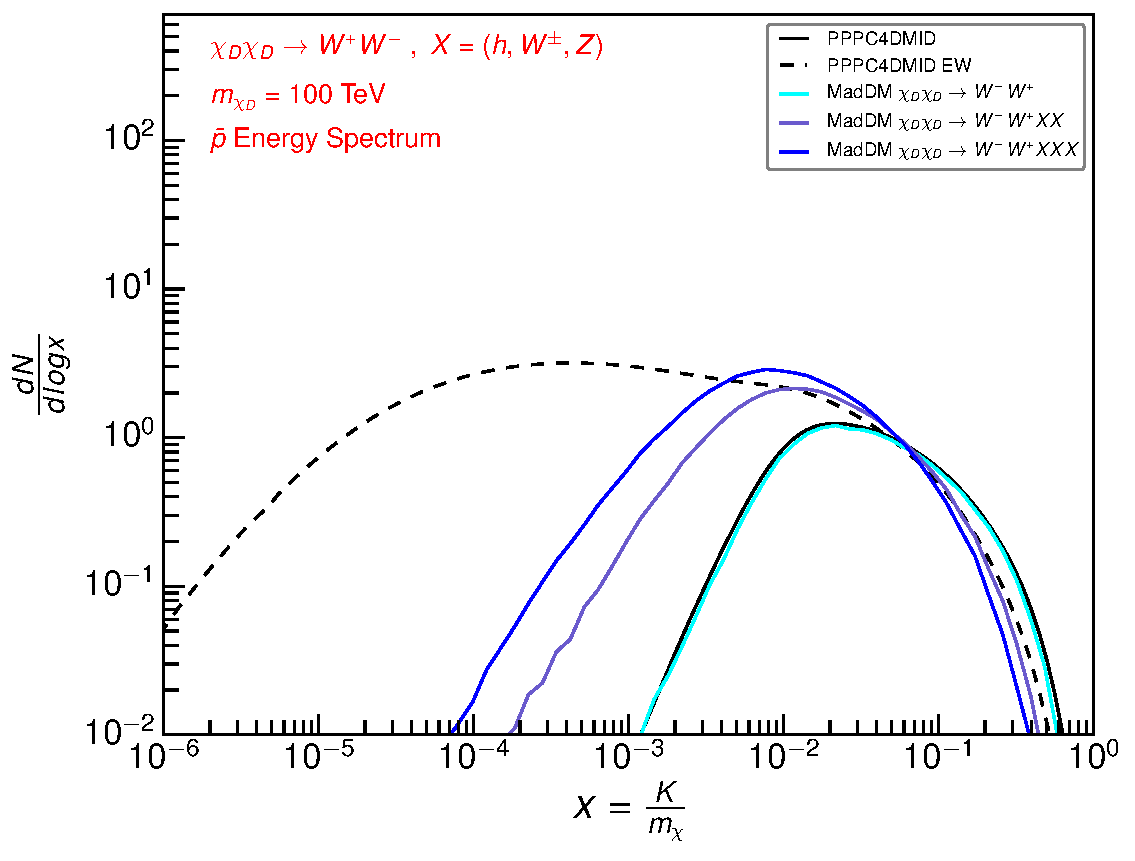
\includegraphics[width=0.49\textwidth]{Fig/100TeV_OLD/OLD_100000_antiprotons_PPPC_Comparison_xdxd_100000.pdf}}
\subfigure
{ 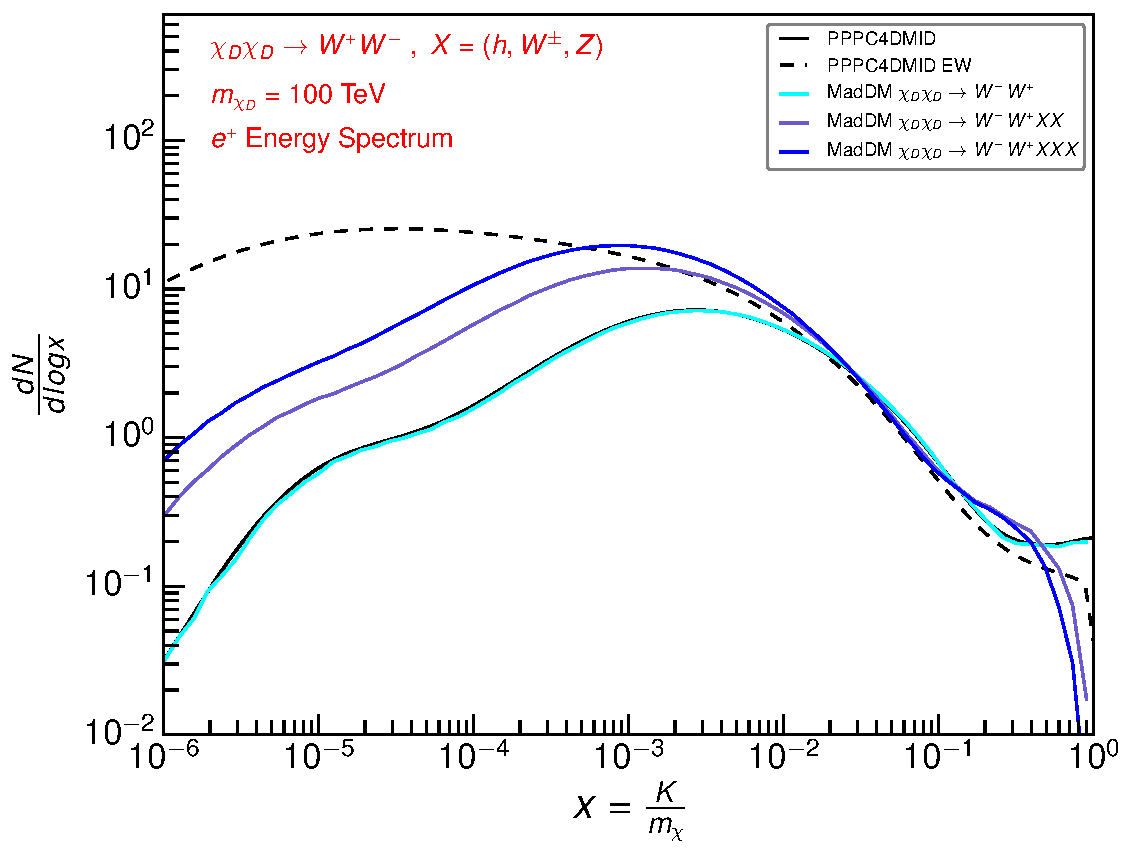
\includegraphics[width=0.49\textwidth]{Fig/100TeV_OLD/OLD_100000_positrons_PPPC_Comparison_xdxd_100000.pdf}}
\subfigure
{ 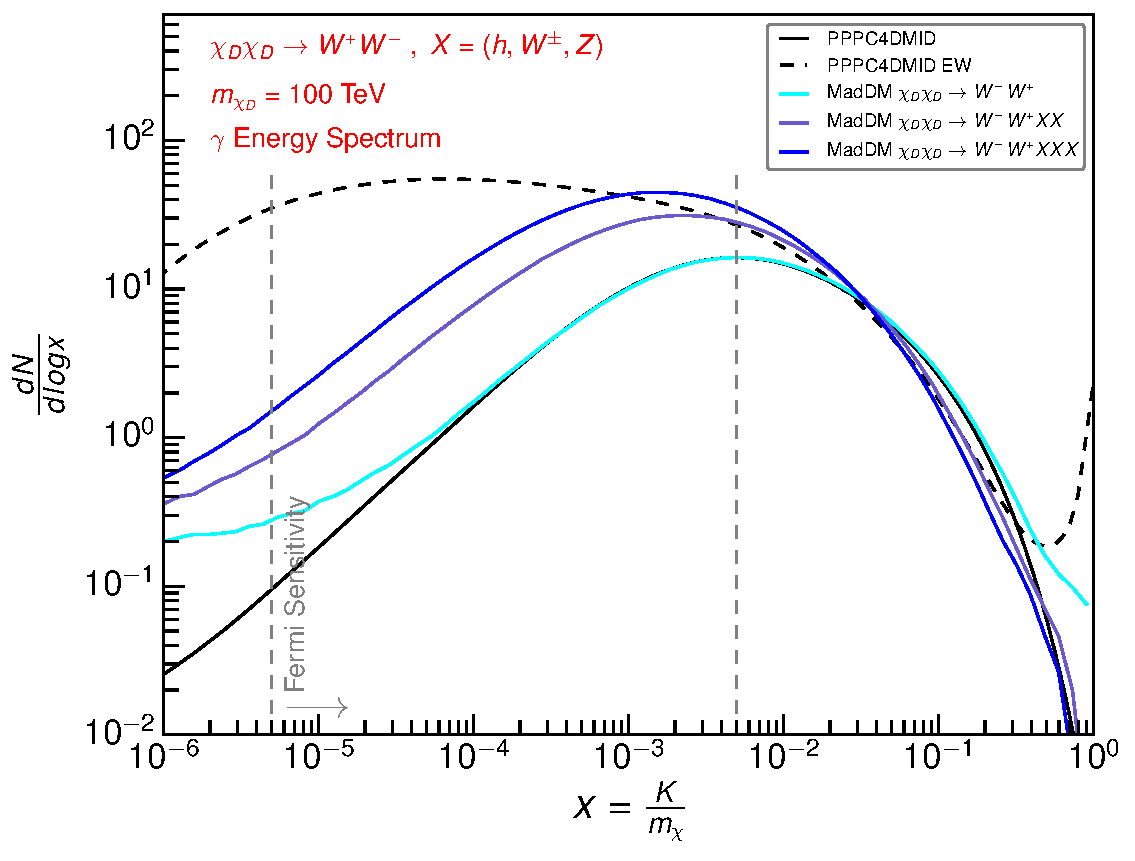
\includegraphics[width=0.49\textwidth]{Fig/100TeV_OLD/OLD_100000_gammas_PPPC_Comparison_xdxd_100000.pdf}}
\subfigure
{ 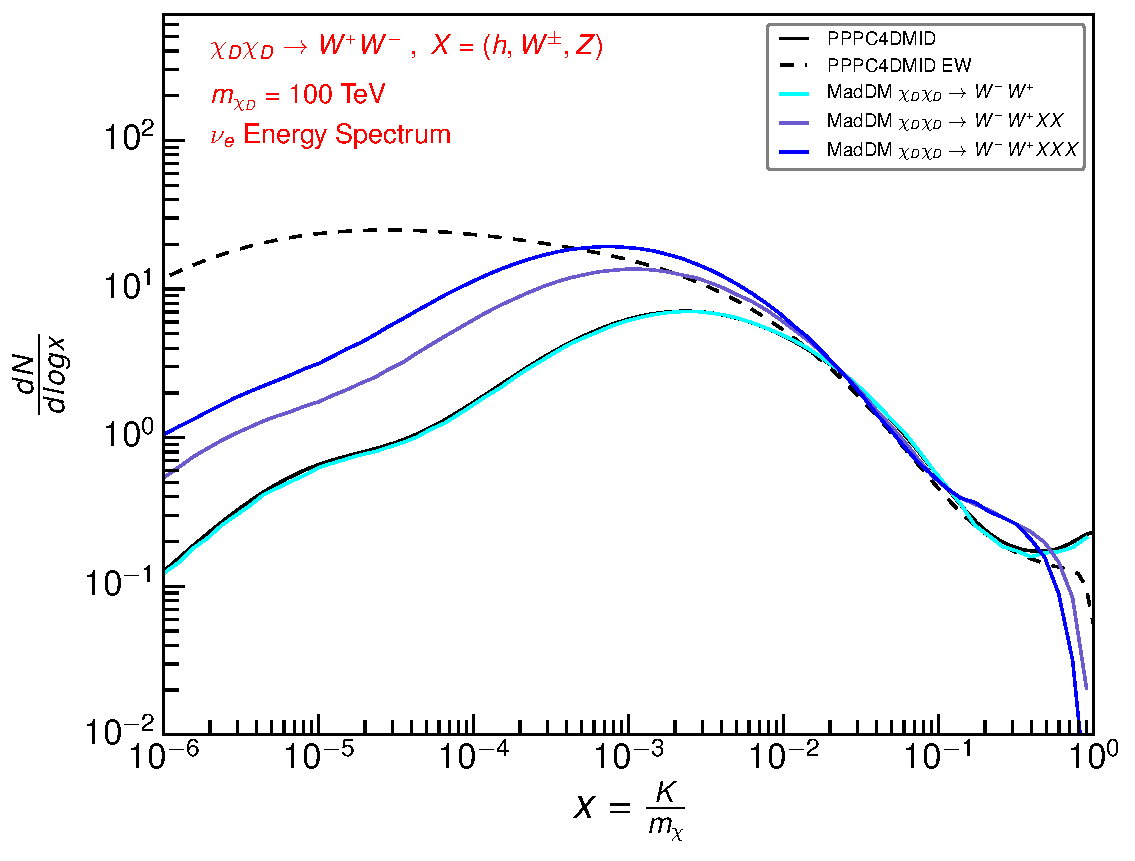
\includegraphics[width=0.49\textwidth]{Fig/100TeV_OLD/OLD_100000_neutrinos_e_PPPC_Comparison_xdxd_100000.pdf}}
\subfigure
{ 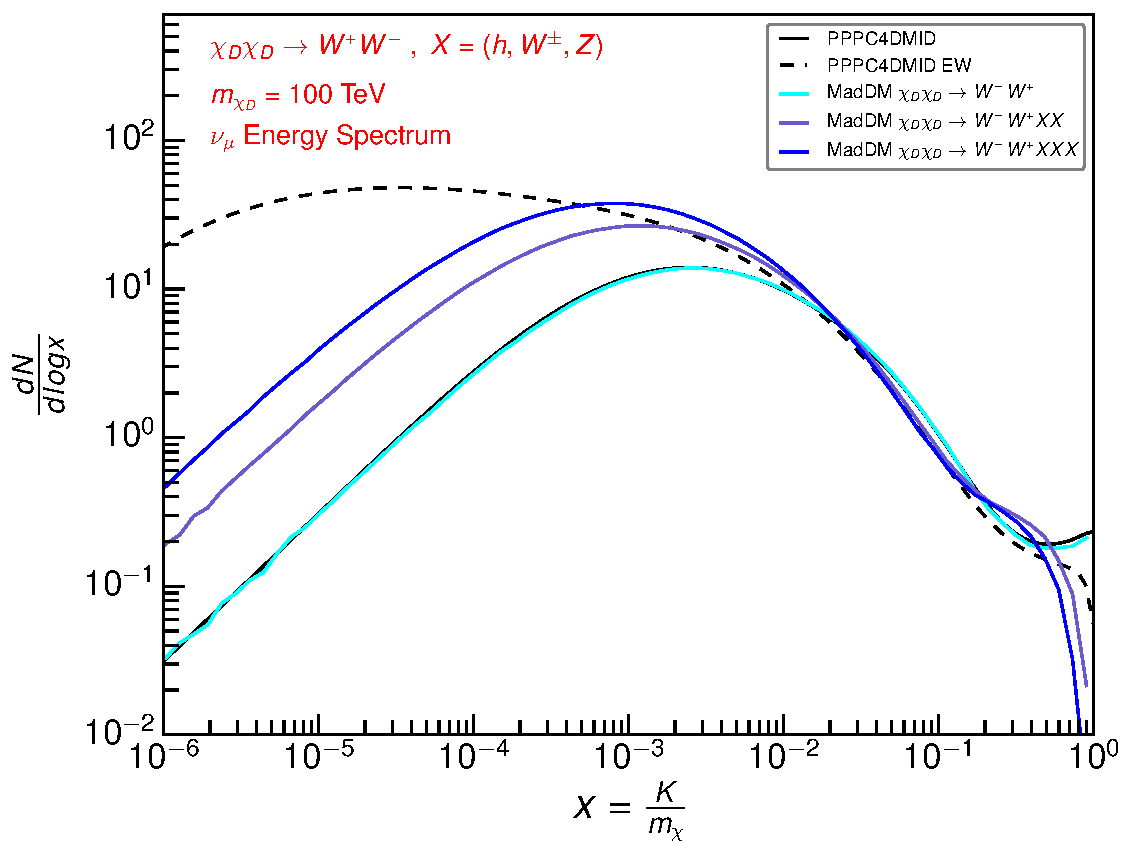
\includegraphics[width=0.49\textwidth]{Fig/100TeV_OLD/OLD_100000_neutrinos_mu_PPPC_Comparison_xdxd_100000.pdf}}
\subfigure
{ 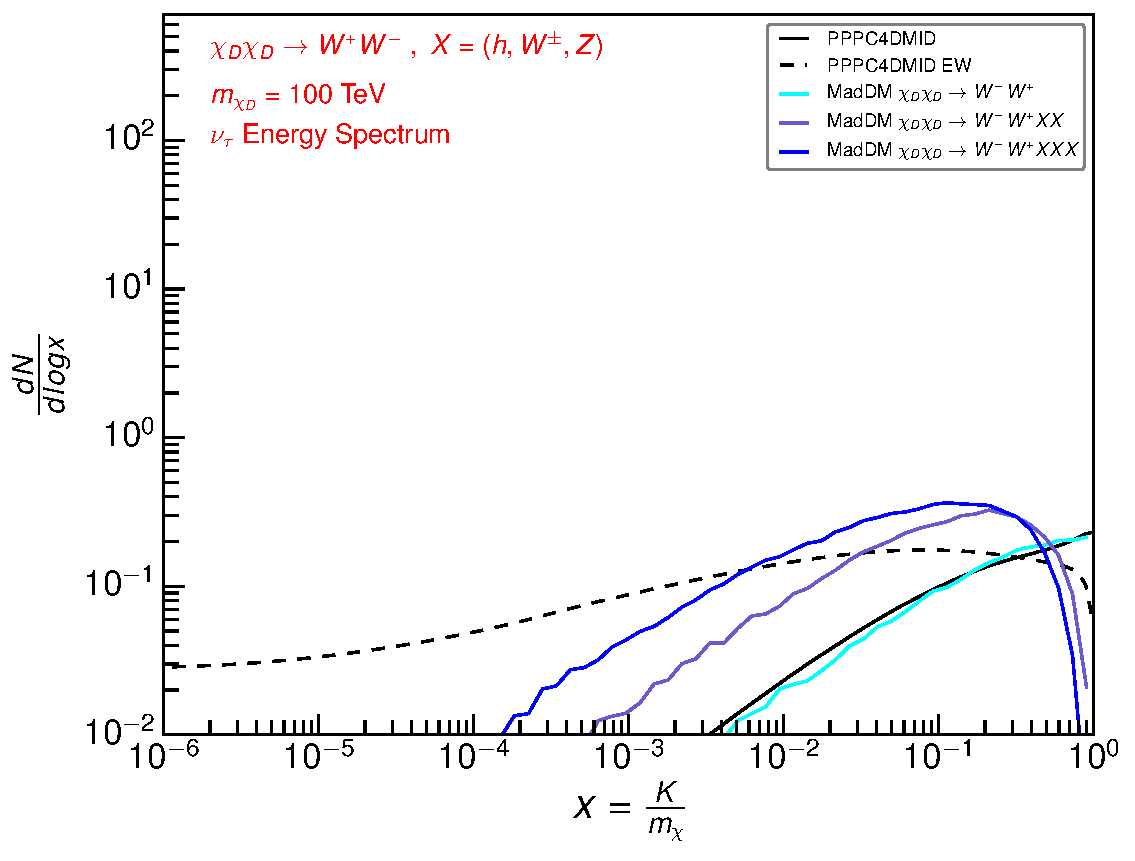
\includegraphics[width=0.49\textwidth]{Fig/100TeV_OLD/OLD_100000_neutrinos_tau_PPPC_Comparison_xdxd_100000.pdf}}
\caption{Energy Spectra for $m_{\chi_D}$ = 100 TeV (Old data)}
\end{figure}
%

\clearpage
\subsection{Spectra for $\chi_D \chi_D \rightarrow Y0 \rightarrow FFFF$}

Here the spectra for the process $\chi_D \chi_D \rightarrow Y0 \rightarrow FFFF$ are shown for $m_{\chi_D}$ = 1 TeV, compared to the \PPPC and \PPPCew~ spectra. To produce the sample, the EW model was modified adding masses to the light quarks and muons, otherwise there is a problem in \MG~when evaluating the cross sections (re-using the same diagrams with masless particles?). I used the value of the muon mass (0.105 GeV) for the light quarks, and 4.5 GeV for the bottoms. \\
Note that this process include also Z bosons, since I did not remove their contribution explicitly form the diagrams, and that all the bosons contributing to the diagrams are on-shell. The presence of the Z/H bosons can account for some of the differences wrt the WW spectra from \PPPC or \PPPCew~.

The model can be found at {\color{blue} \url{https://github.com/fambrogi/MadDM/tree/master/EW_Study/EW_Model_FermionMass}}, while the complete banner can be found in {\color{blue} \url{https://github.com/fambrogi/MadDM/blob/master/EW_Study/Banners/xdxd_Y0_FFFF_1TeV_banner.dat} }.
\\


\MG~ Process:
\begin{verbatim}
import model DMsimp_s_spin0_EW_MM
define F = ve vm vt e- mu- ve~ vm~ vt~ e+ mu+ t t~ u c d s b u~ c~ d~ \
s~ b~ ta- ta+
generate xd xd~ > y0 > F F F F
output xdxd_Y0_FFFF
\end{verbatim}
%
\\


Pythia8 cards commands:
\begin{verbatim}
TimeShower:weakShower = on (or off)
WeakShower:singleEmission = off
\end{verbatim}



\begin{figure}[!b]
\centering
\subfigure
{ 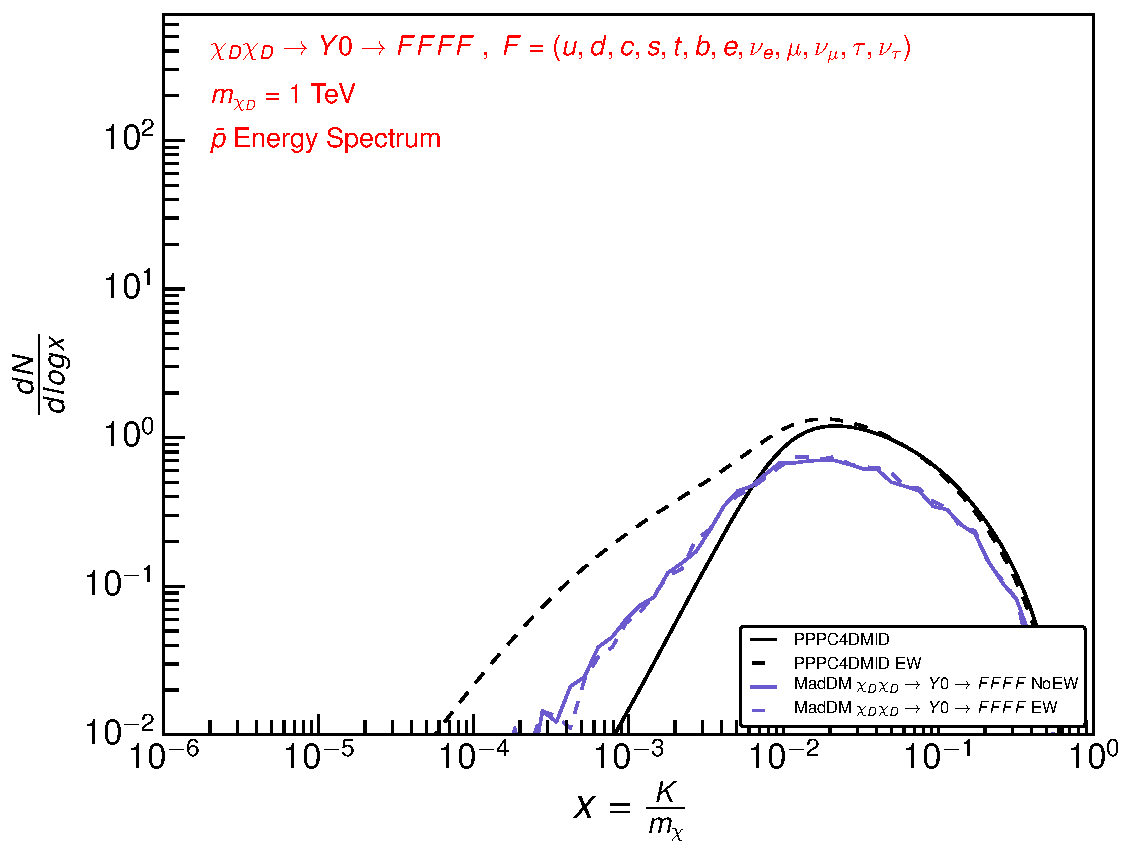
\includegraphics[width=0.49\textwidth]{Fig/xdxd_Y0/1_antiprotons_FFFF_xdxd_1.pdf}}
\subfigure
{ 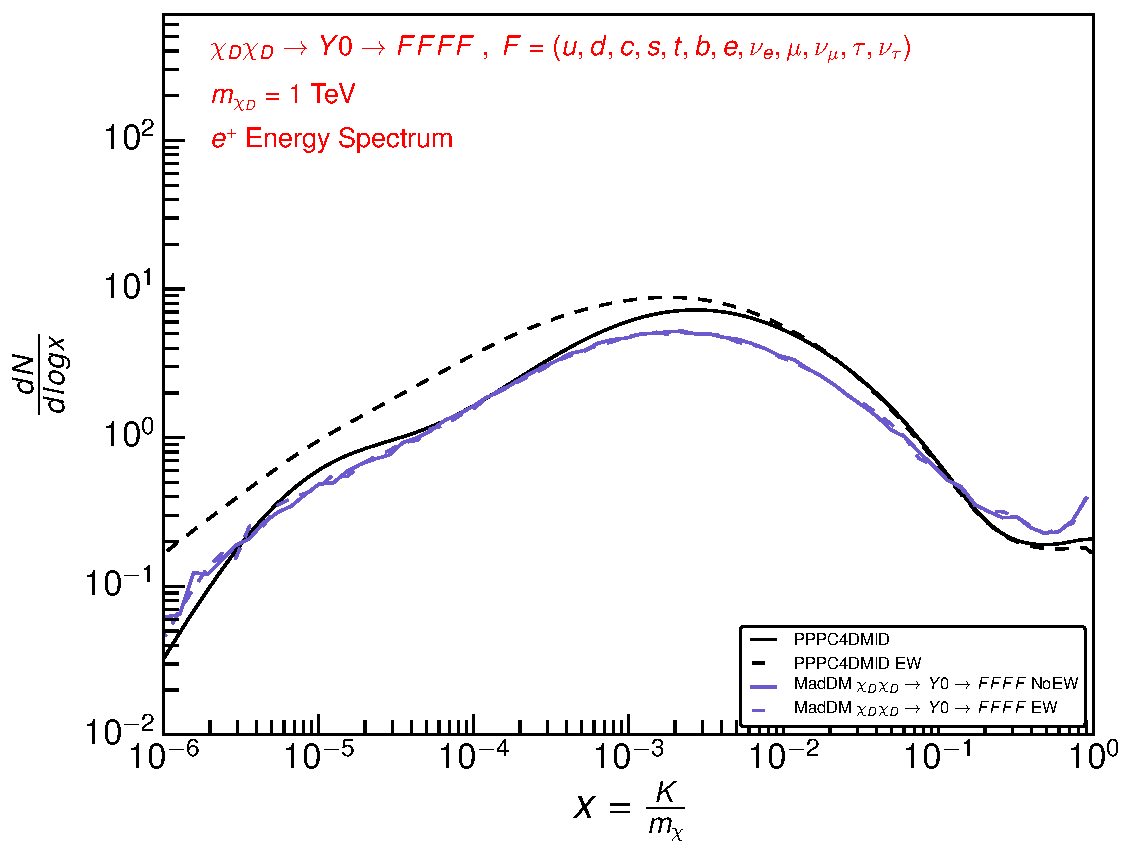
\includegraphics[width=0.49\textwidth]{Fig/xdxd_Y0/1_positrons_FFFF_xdxd_1.pdf}}
\subfigure
{ 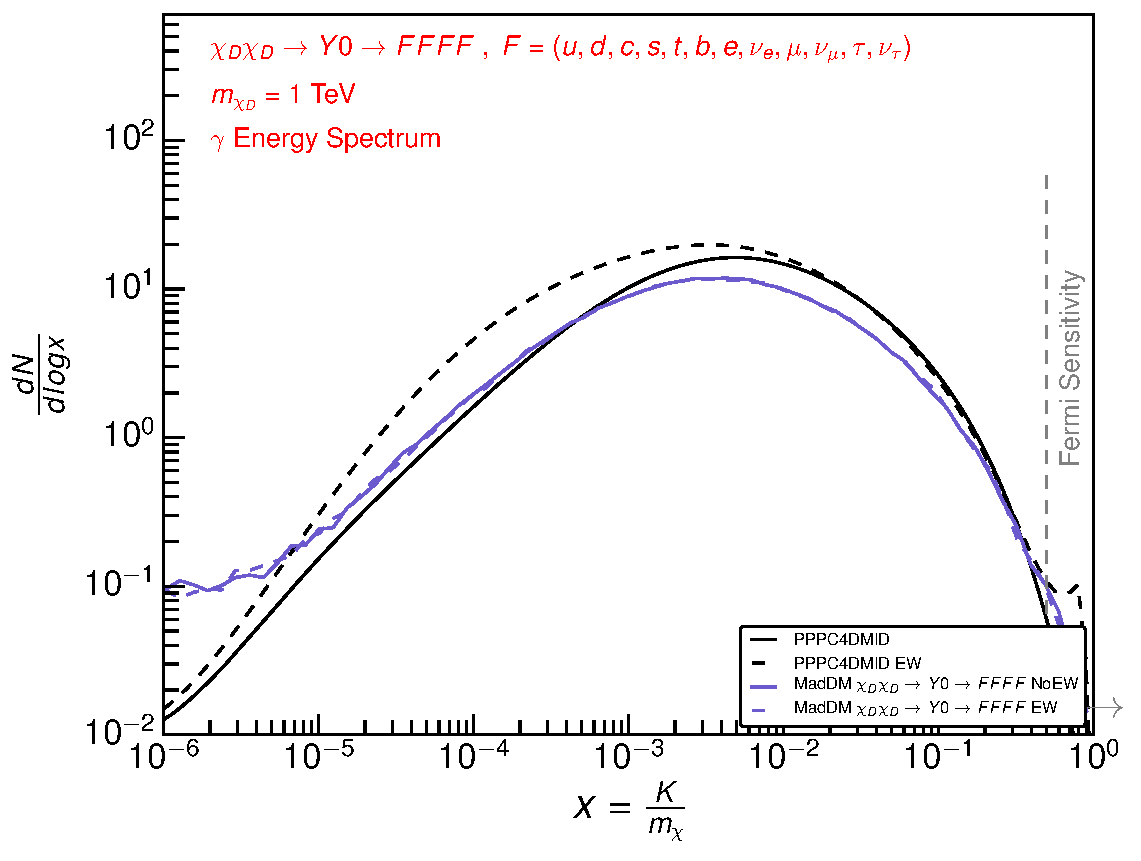
\includegraphics[width=0.49\textwidth]{Fig/xdxd_Y0/1_gammas_FFFF_xdxd_1.pdf}}
\subfigure
{ 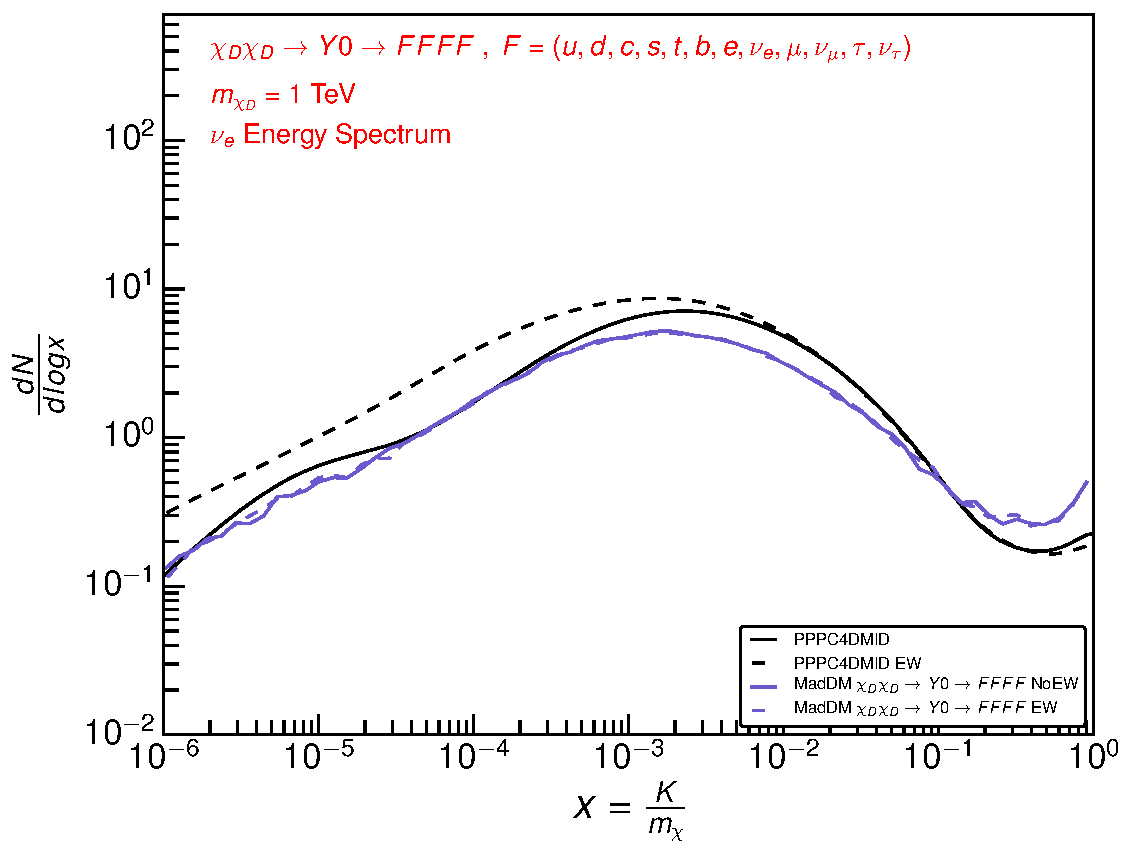
\includegraphics[width=0.49\textwidth]{Fig/xdxd_Y0/1_neutrinos_e_FFFF_xdxd_1.pdf}}
\subfigure
{ 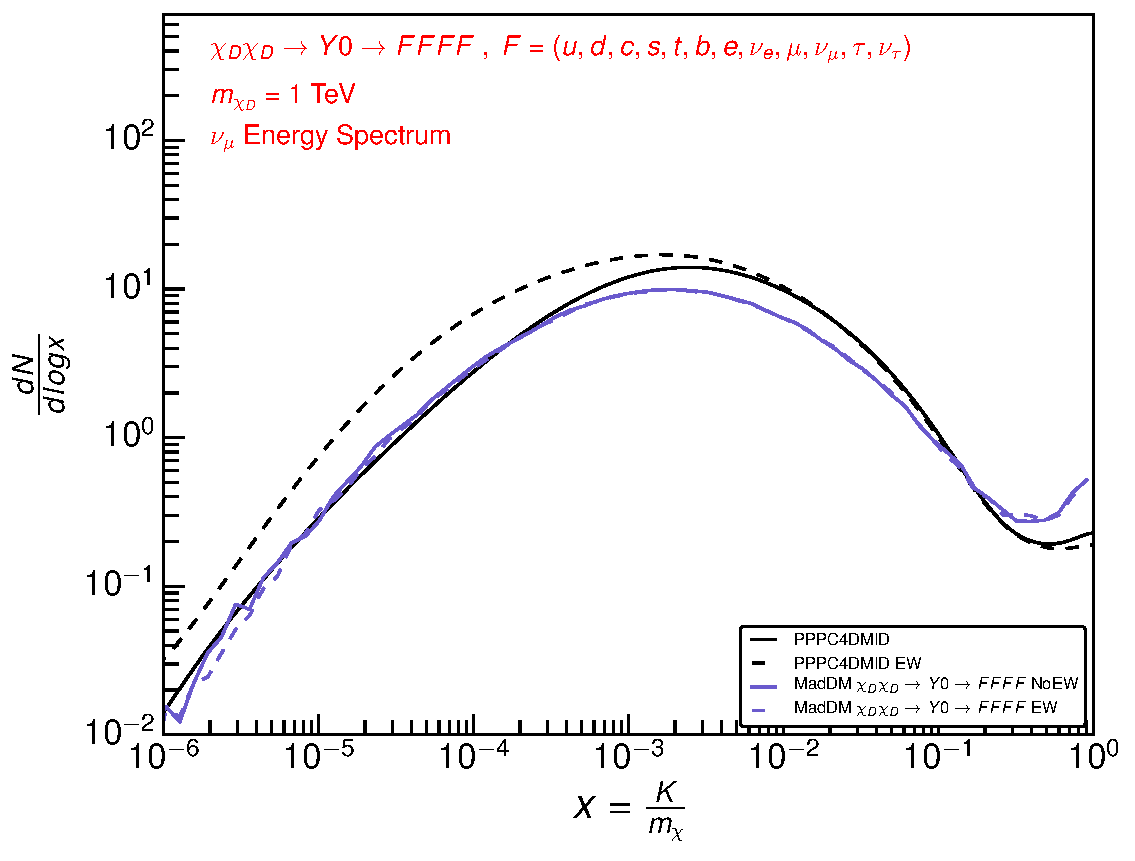
\includegraphics[width=0.49\textwidth]{Fig/xdxd_Y0/1_neutrinos_mu_FFFF_xdxd_1.pdf}}
\subfigure
{ 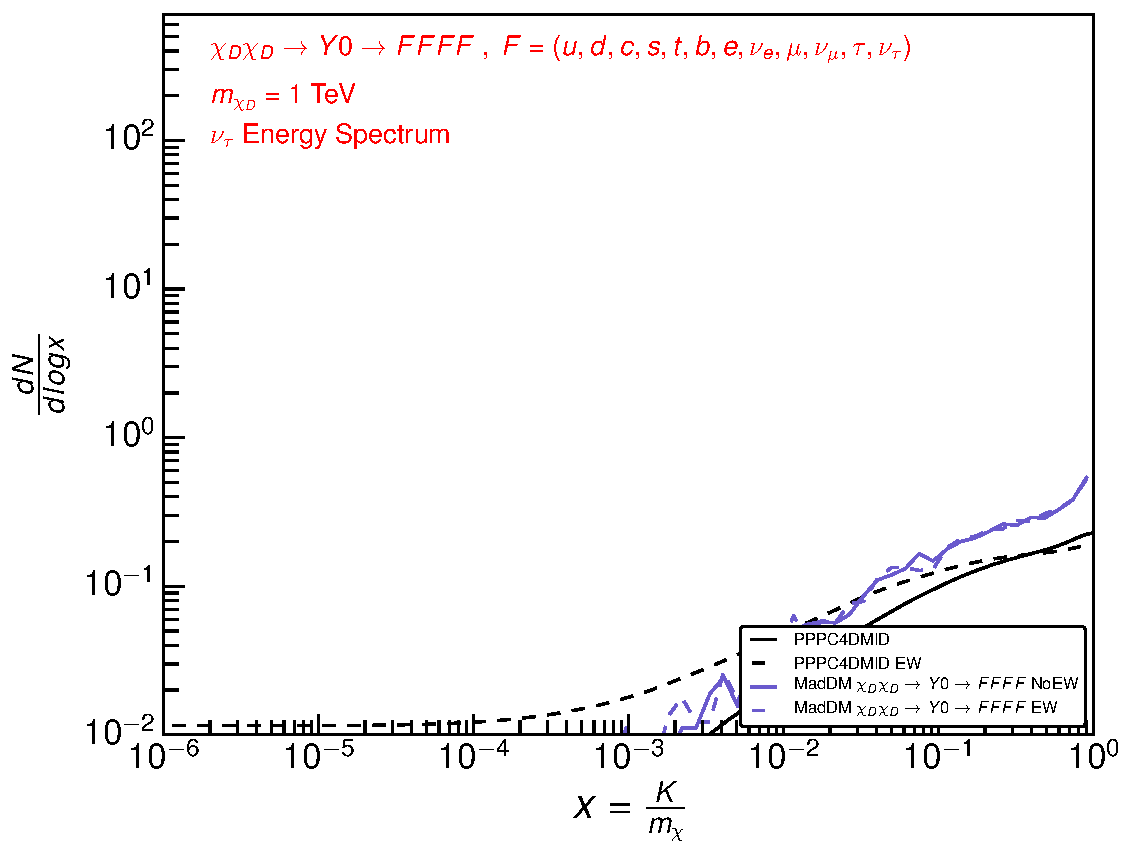
\includegraphics[width=0.49\textwidth]{Fig/xdxd_Y0/1_neutrinos_tau_FFFF_xdxd_1.pdf}}
\caption{Energy Spectra for $m_{\chi_D}$ = 1 TeV for the process $\chi_D \chi_D \rightarrow Y0 \rightarrow FFFF$. The label "EW" and "NoEW" in the MadDM samples mean respectively samples produced with or without the EW corrections in Pythia8.}
\end{figure}


\clearpage
\subsection{Spectra for $\chi_D \chi_D \rightarrow Y0 \rightarrow FFFF$ with off-shell W and no Z}
The spectra in Fig. \ref{woff_1},\ref{woff_10},\ref{woff_100} were produced with the following \MG~processes:
\begin{verbatim}
import model DMsimp_s_spin0_EW_WithMass
define F = ve vm vt e- mu- ve~ vm~ vt~ e+ mu+ t t~ u c d s b u~ c~ d~ \
s~ b~ ta- ta+
generate xd xd~ > F F F F $ w- w+ / z
output xdxd_FFFF_WoffNoZ
\end{verbatim}
so, differently from the previous case, the $W^{\pm }$ bosons are required to be off-shell, and the $Z$ bosons are removed from the diagrams. In addition, the spectra obtained with the removal of intermediate $Z$ bosons only are shown.
\clearpage
\subsubsection{ $m_{\chi_D}$ = 1 TeV}
\begin{figure}[!b]
\centering
\subfigure
{ 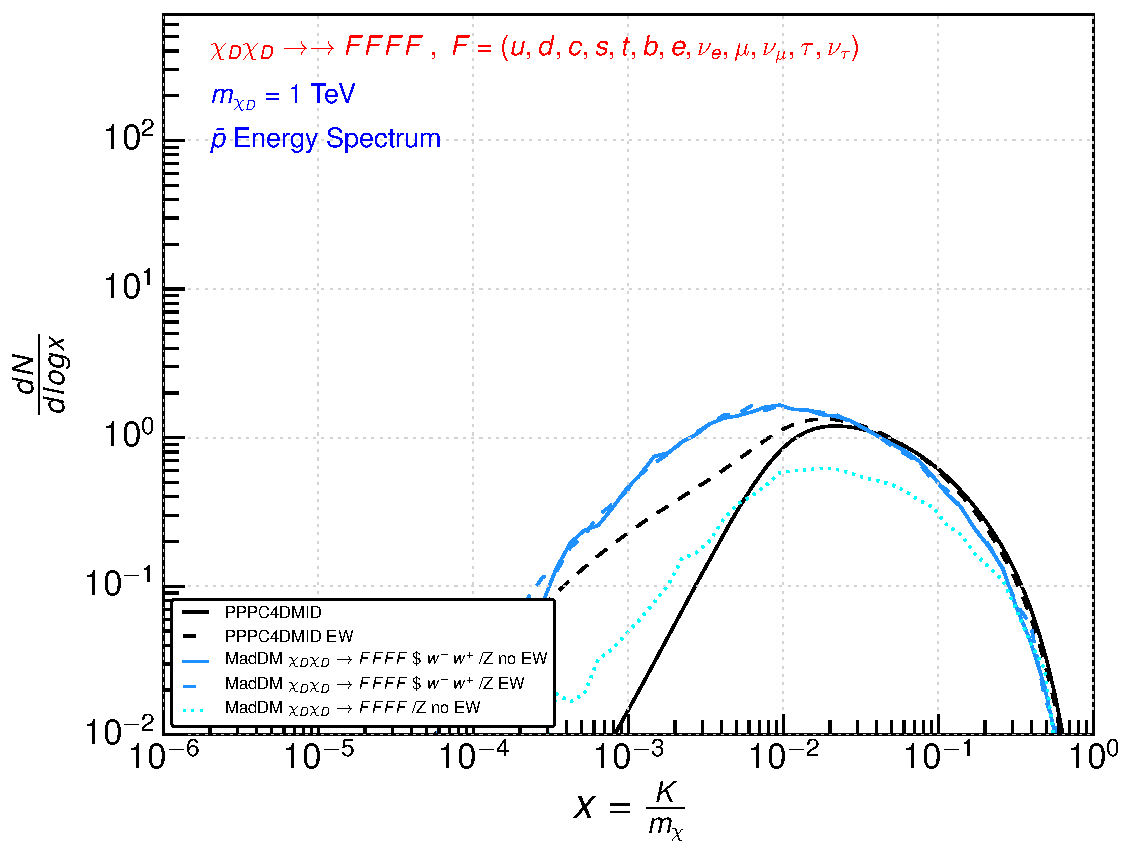
\includegraphics[width=0.49\textwidth]{Fig/xdxd_FFFF_WZ/1_antiprotons_FFFF_1.pdf}}
\subfigure
{ 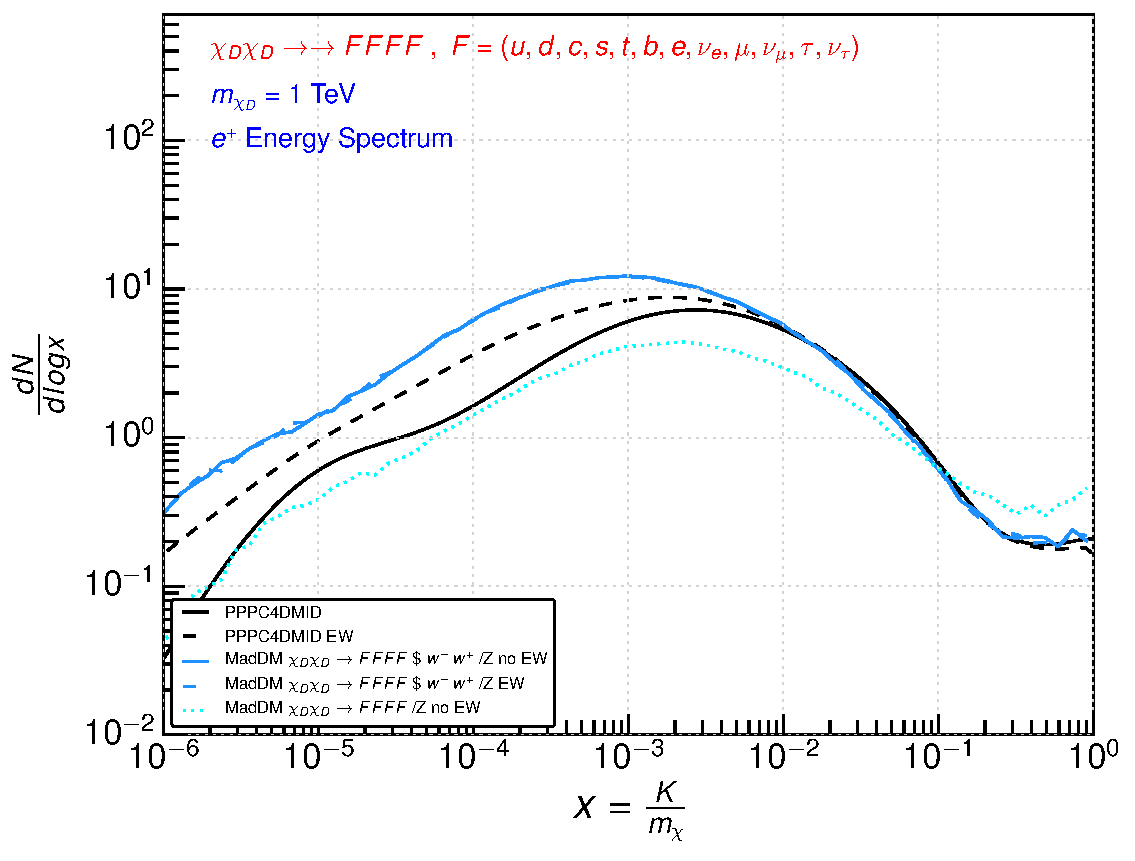
\includegraphics[width=0.49\textwidth]{Fig/xdxd_FFFF_WZ/1_positrons_FFFF_1.pdf}}
\subfigure
{ 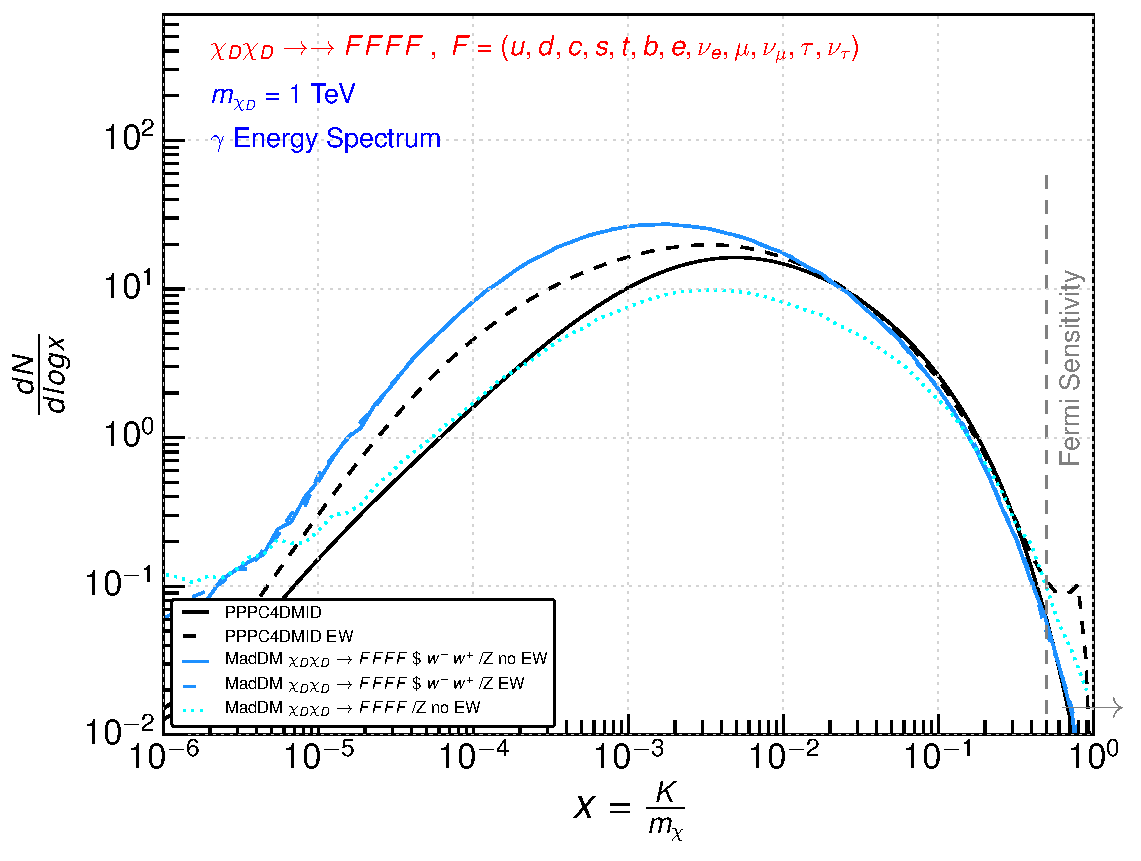
\includegraphics[width=0.49\textwidth]{Fig/xdxd_FFFF_WZ/1_gammas_FFFF_1.pdf}}
\subfigure
{ 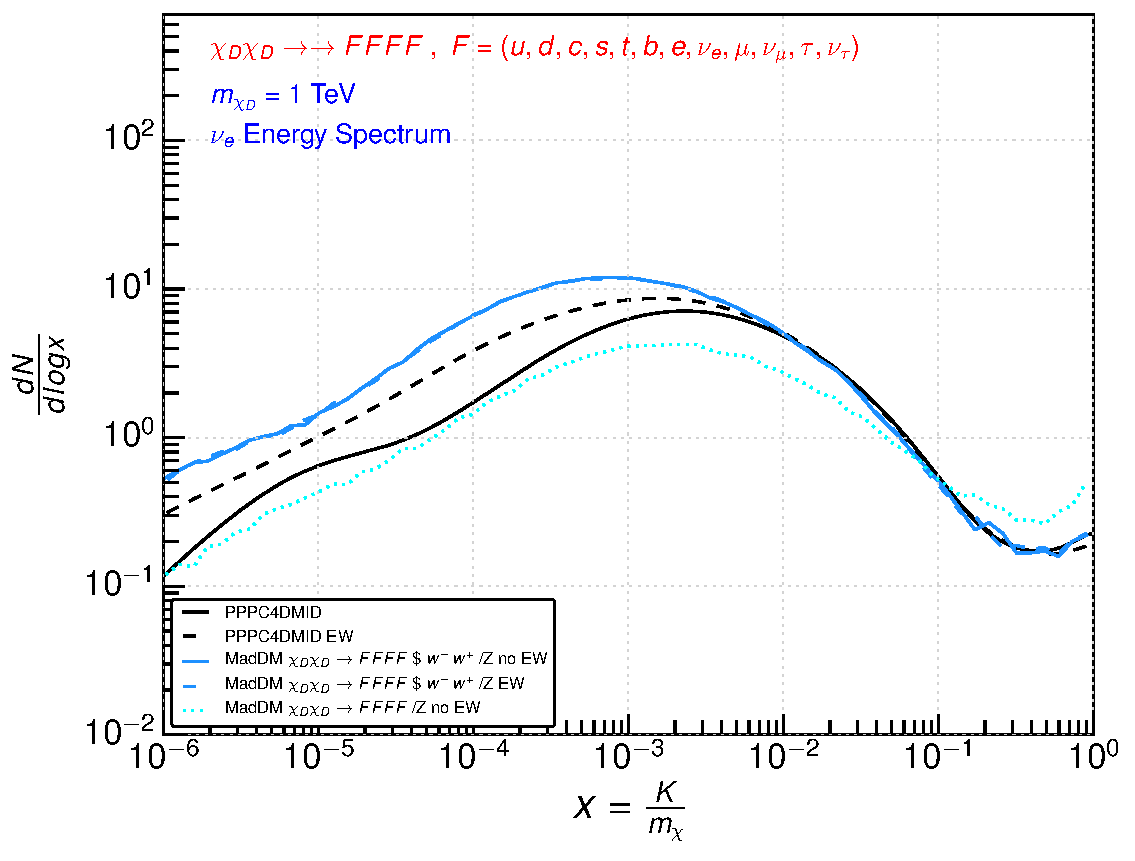
\includegraphics[width=0.49\textwidth]{Fig/xdxd_FFFF_WZ/1_neutrinos_e_FFFF_1.pdf}}
\subfigure
{ 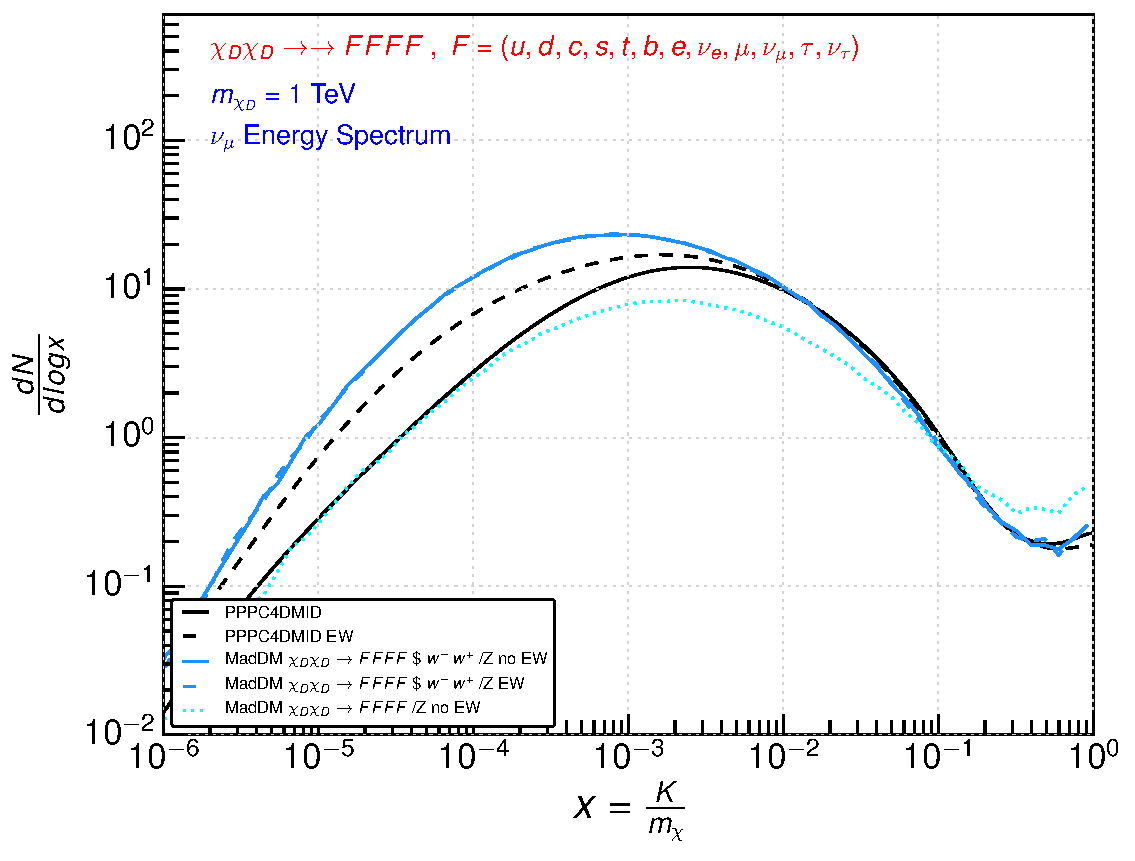
\includegraphics[width=0.49\textwidth]{Fig/xdxd_FFFF_WZ/1_neutrinos_mu_FFFF_1.pdf}}
\subfigure
{ 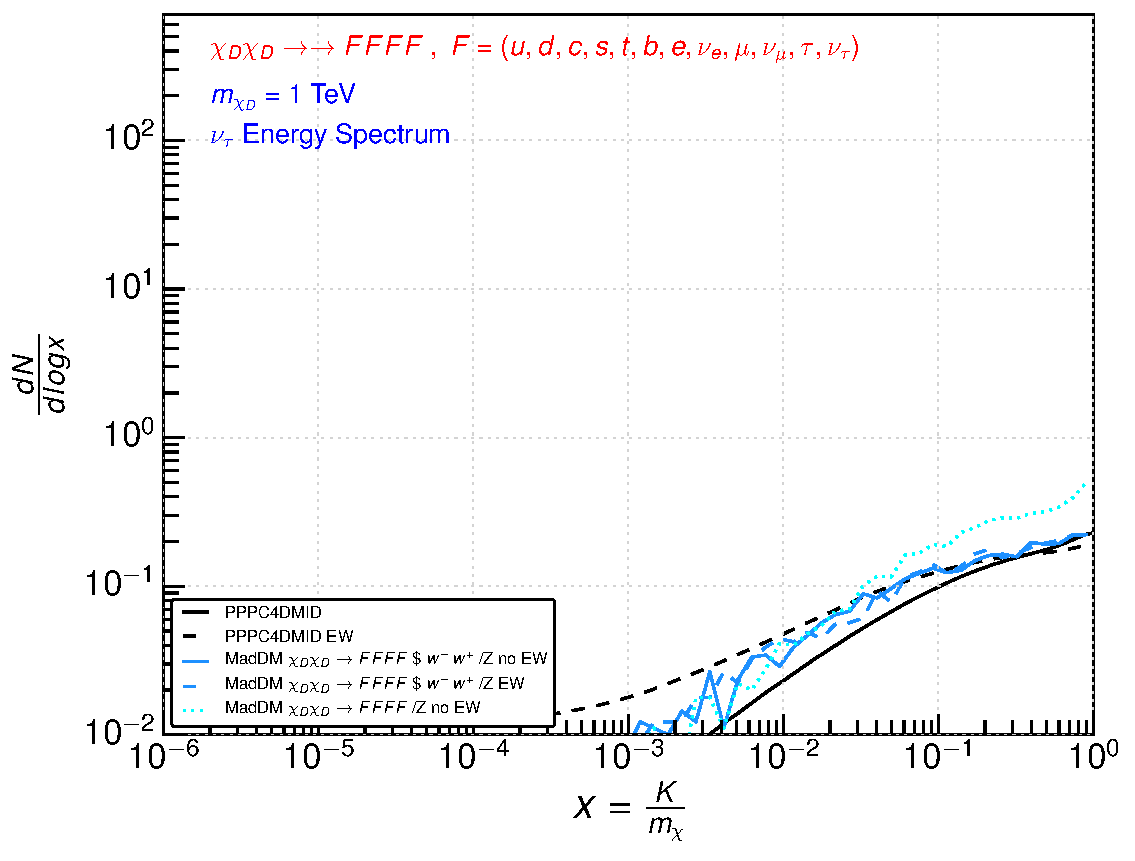
\includegraphics[width=0.49\textwidth]{Fig/xdxd_FFFF_WZ/1_neutrinos_tau_FFFF_1.pdf}}
\caption{Energy Spectra for $m_{\chi_D}$ = 1 TeV for the process $\chi_D \chi_D \rightarrow Y0 \rightarrow FFFF \$w^- w^+ /Z $, for $m_{\chi_D}$ = 1 TeV. The label "EW" and "NoEW" in the MadDM samples mean respectively samples produced with or without the EW corrections in Pythia8.}
\label{woff_1}
\end{figure}


\clearpage
\subsubsection{ $m_{\chi_D}$ = 10 TeV}
\begin{figure}[!b]
\centering
\subfigure
{ 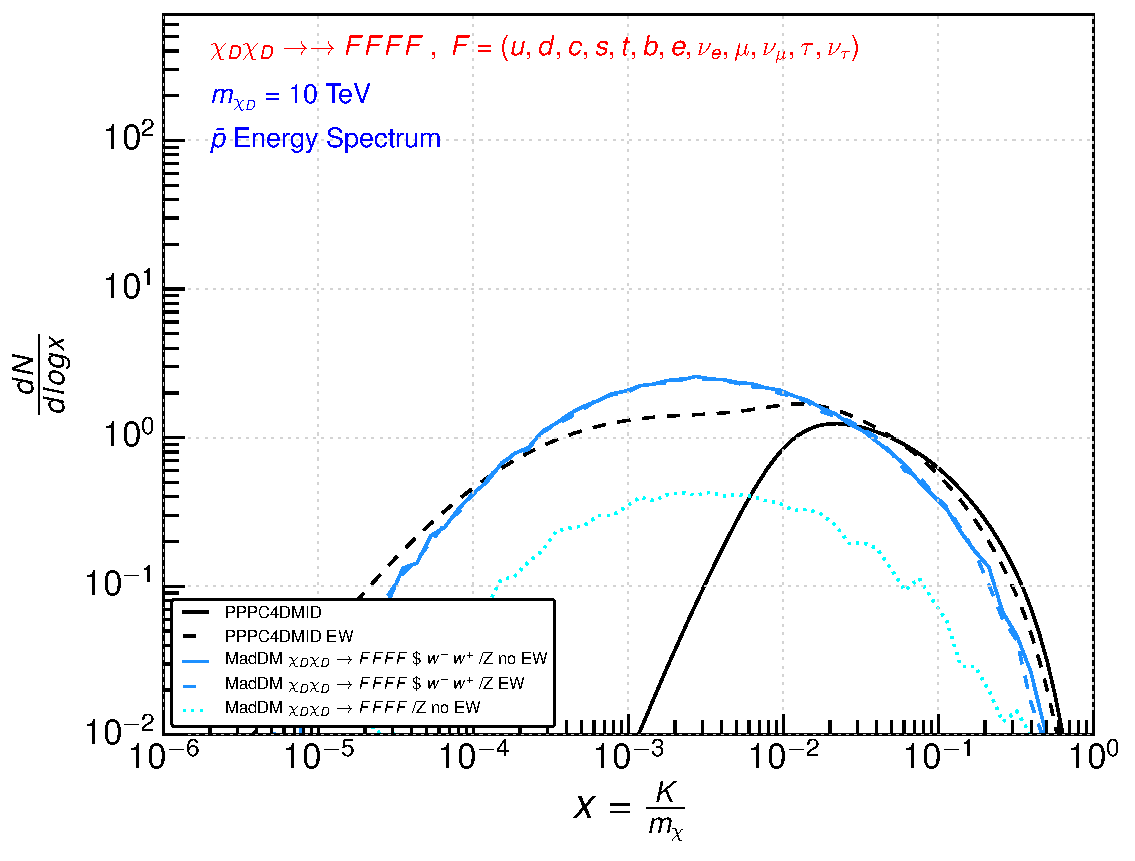
\includegraphics[width=0.49\textwidth]{Fig/xdxd_FFFF_WZ/10_antiprotons_FFFF_10.pdf}}
\subfigure
{ 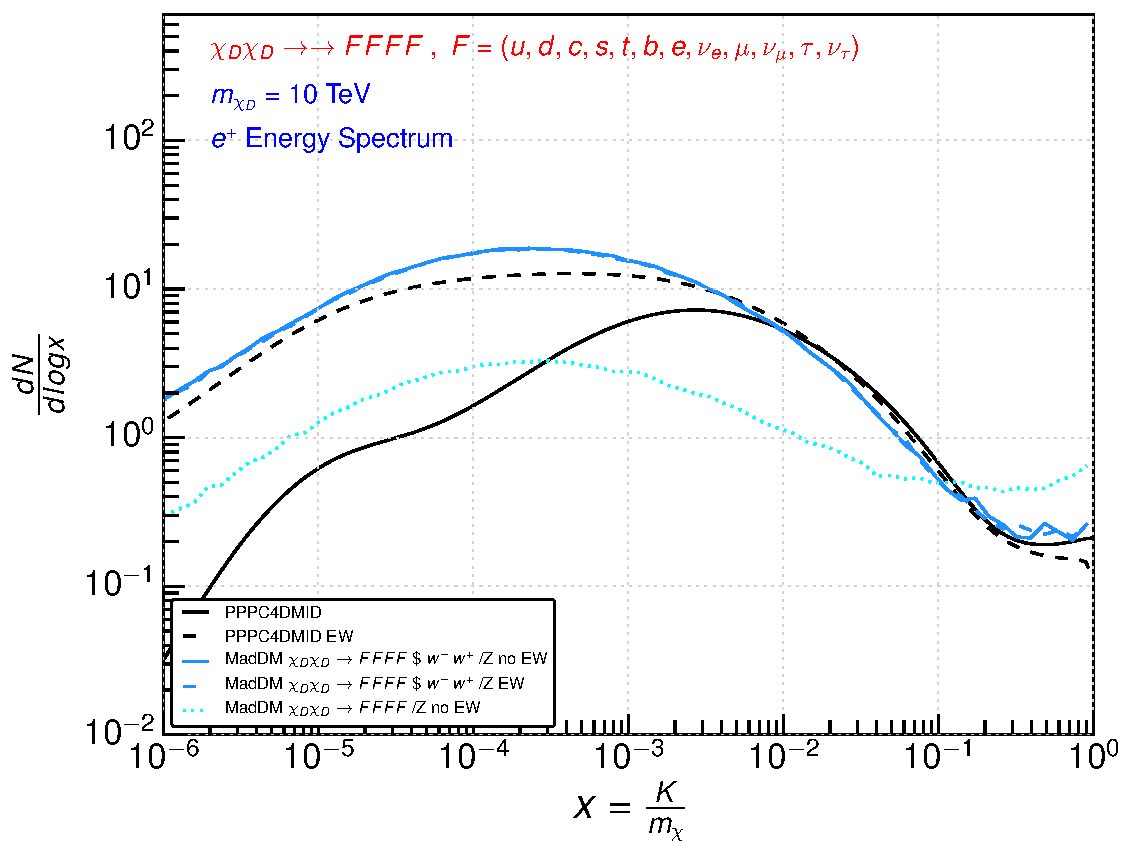
\includegraphics[width=0.49\textwidth]{Fig/xdxd_FFFF_WZ/10_positrons_FFFF_10.pdf}}
\subfigure
{ 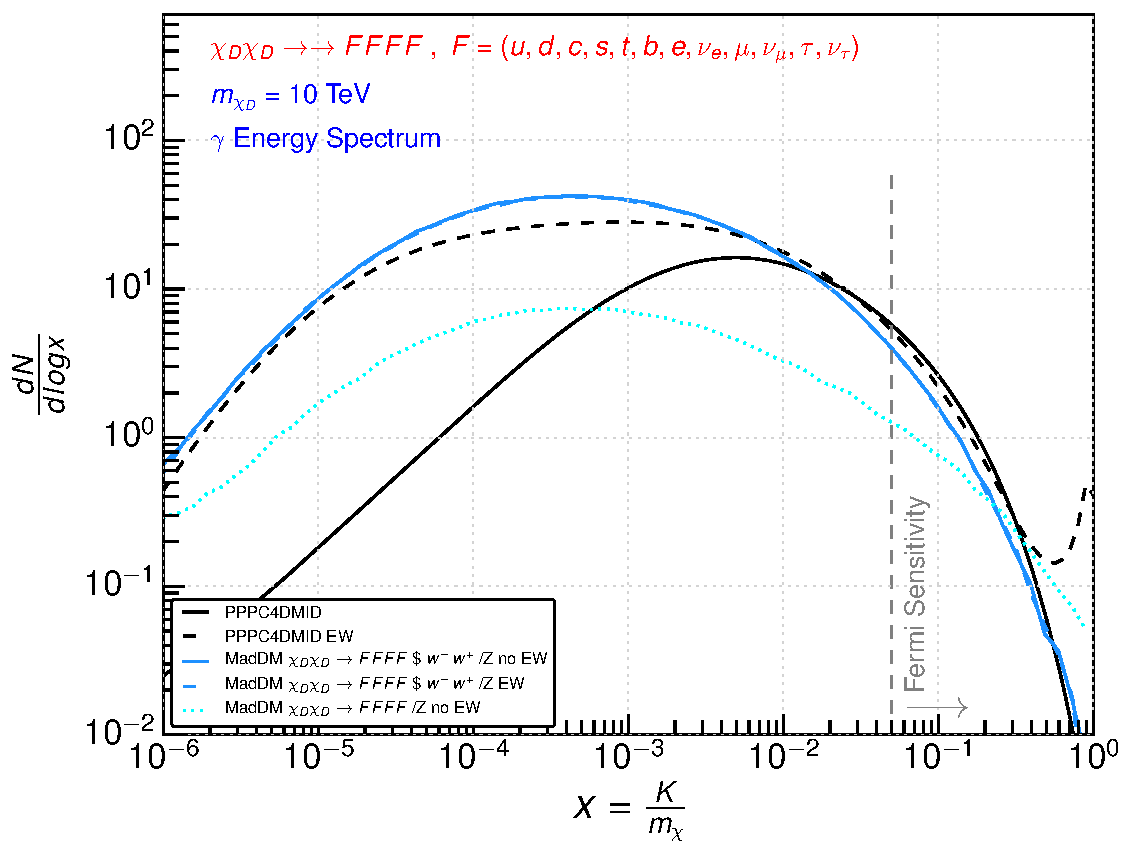
\includegraphics[width=0.49\textwidth]{Fig/xdxd_FFFF_WZ/10_gammas_FFFF_10.pdf}}
\subfigure
{ 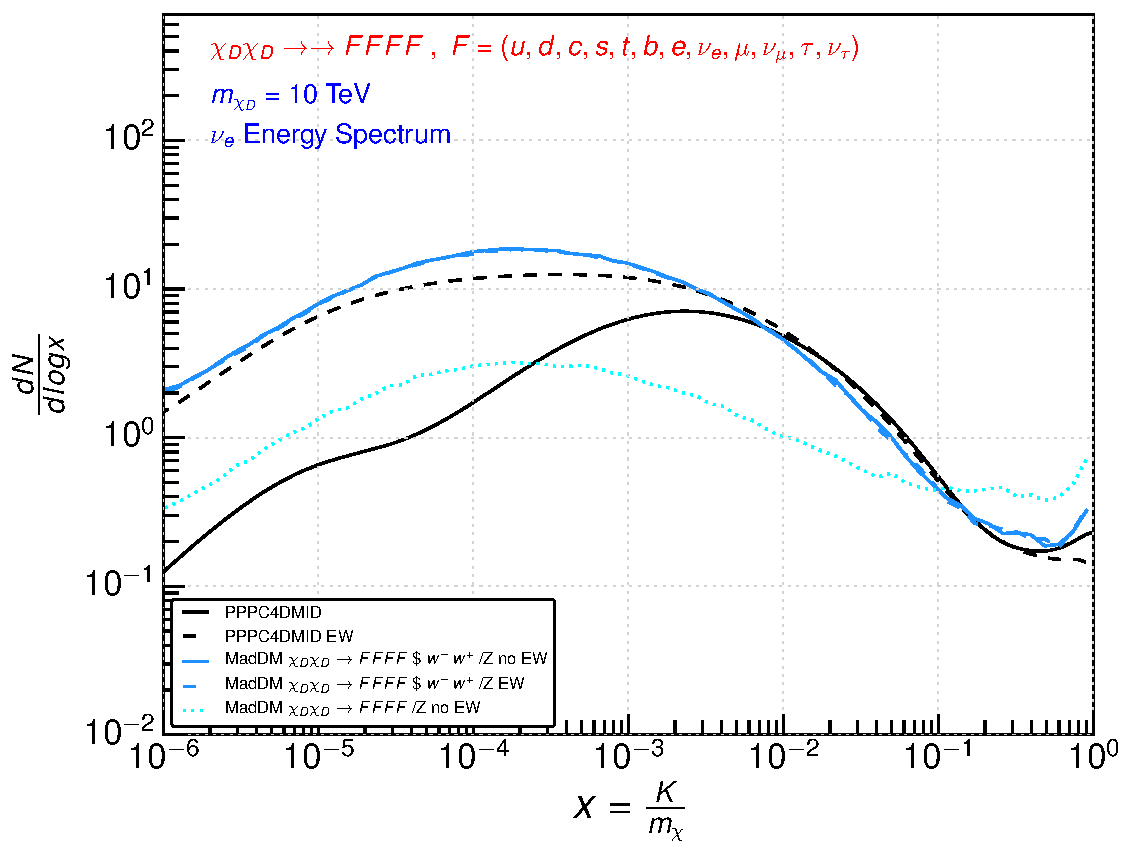
\includegraphics[width=0.49\textwidth]{Fig/xdxd_FFFF_WZ/10_neutrinos_e_FFFF_10.pdf}}
\subfigure
{ 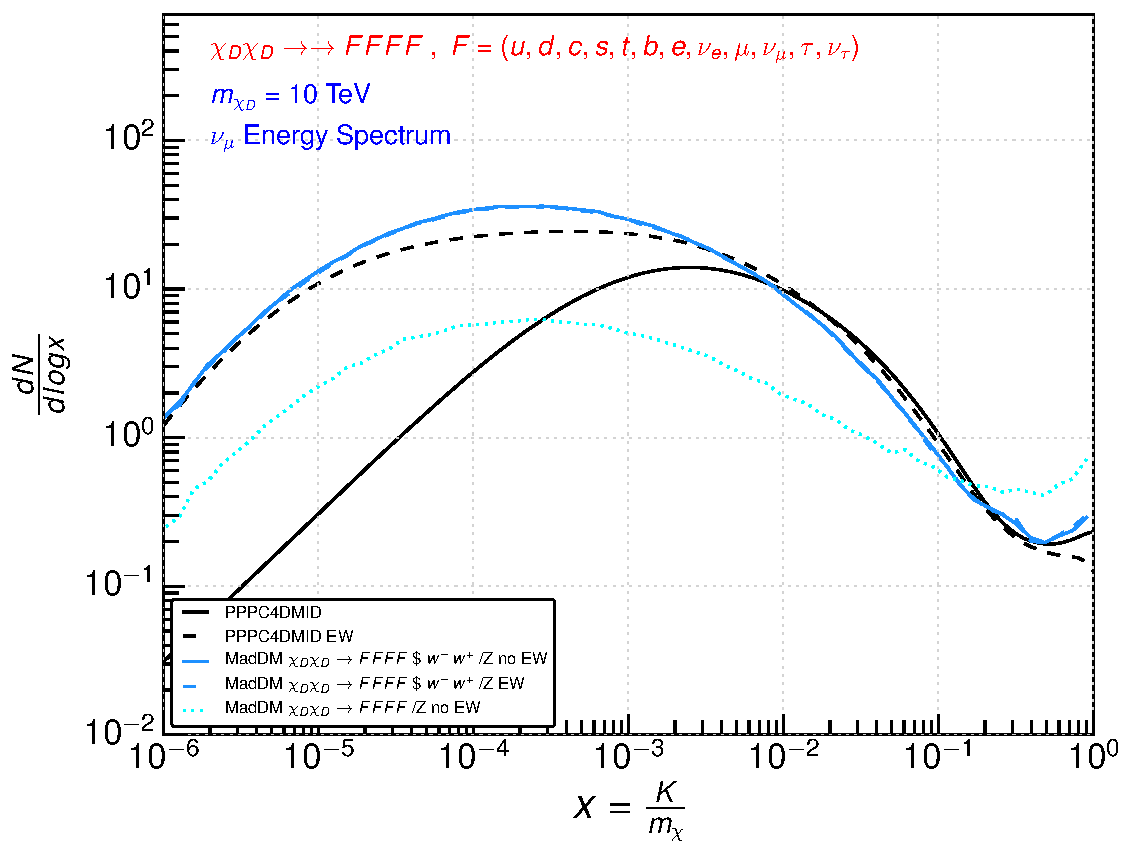
\includegraphics[width=0.49\textwidth]{Fig/xdxd_FFFF_WZ/10_neutrinos_mu_FFFF_10.pdf}}
\subfigure
{ 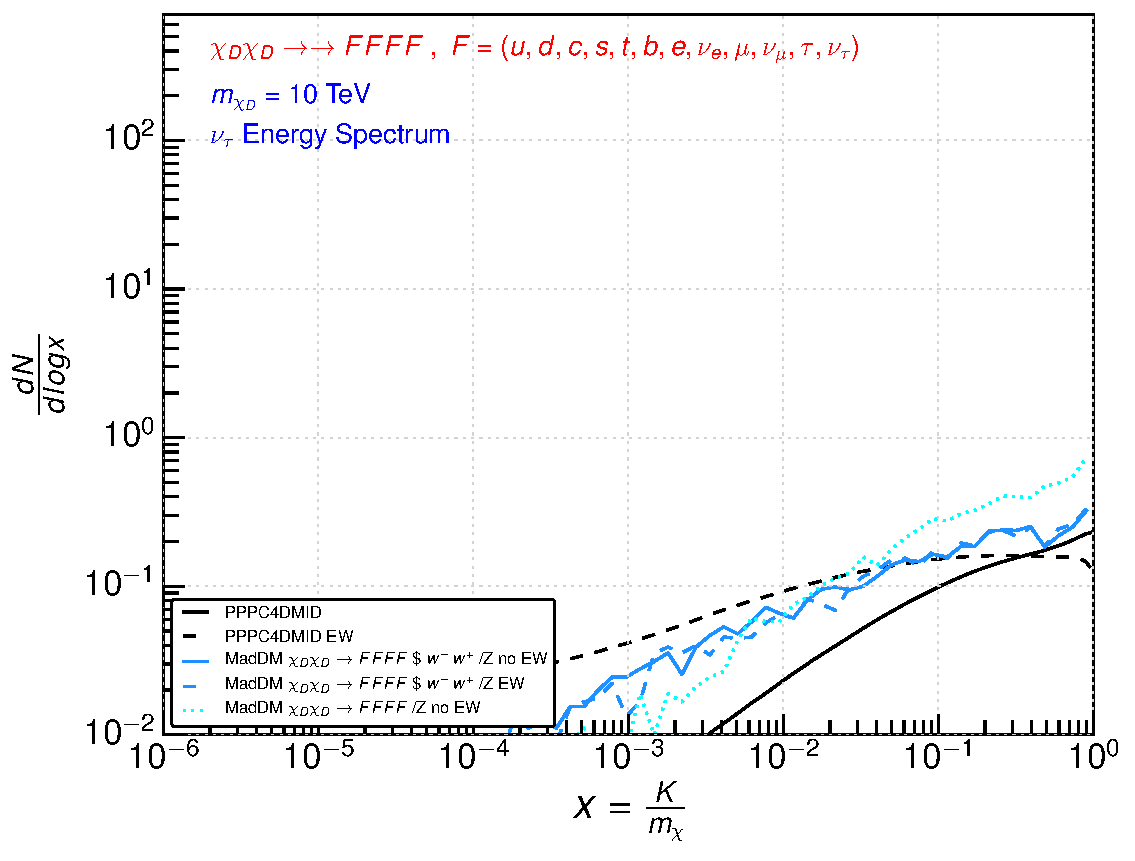
\includegraphics[width=0.49\textwidth]{Fig/xdxd_FFFF_WZ/10_neutrinos_tau_FFFF_10.pdf}}
\caption{Energy Spectra for $m_{\chi_D}$ = 10 TeV for the process $\chi_D \chi_D \rightarrow Y0 \rightarrow FFFF \$w^- w^+ /Z $, for $m_{\chi_D}$ = 1 TeV. The label "EW" and "NoEW" in the MadDM samples mean respectively samples produced with or without the EW corrections in Pythia8.}
\label{woff_10}
\end{figure}

\clearpage
\subsubsection{ $m_{\chi_D}$ = 100 TeV}
\begin{figure}[!b]
\centering
\subfigure
{ 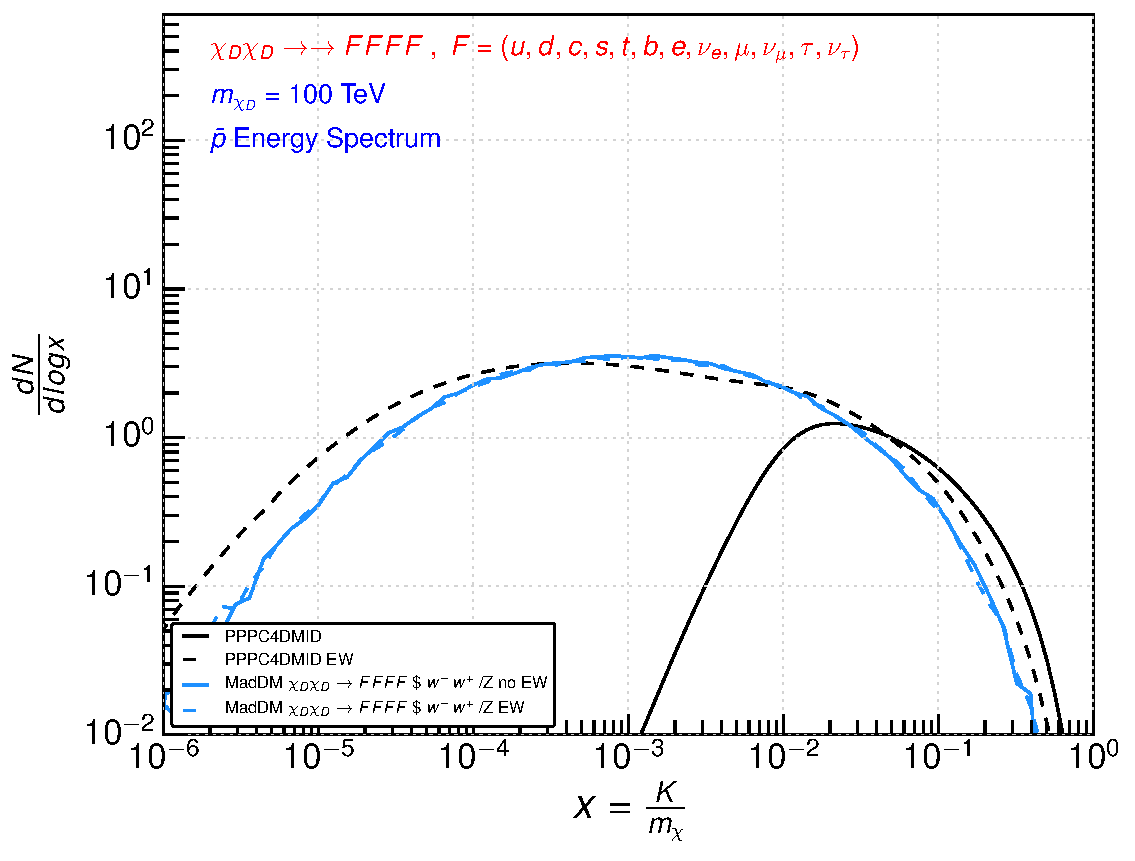
\includegraphics[width=0.49\textwidth]{Fig/xdxd_FFFF_WZ/100_antiprotons_FFFF_100.pdf}}
\subfigure
{ 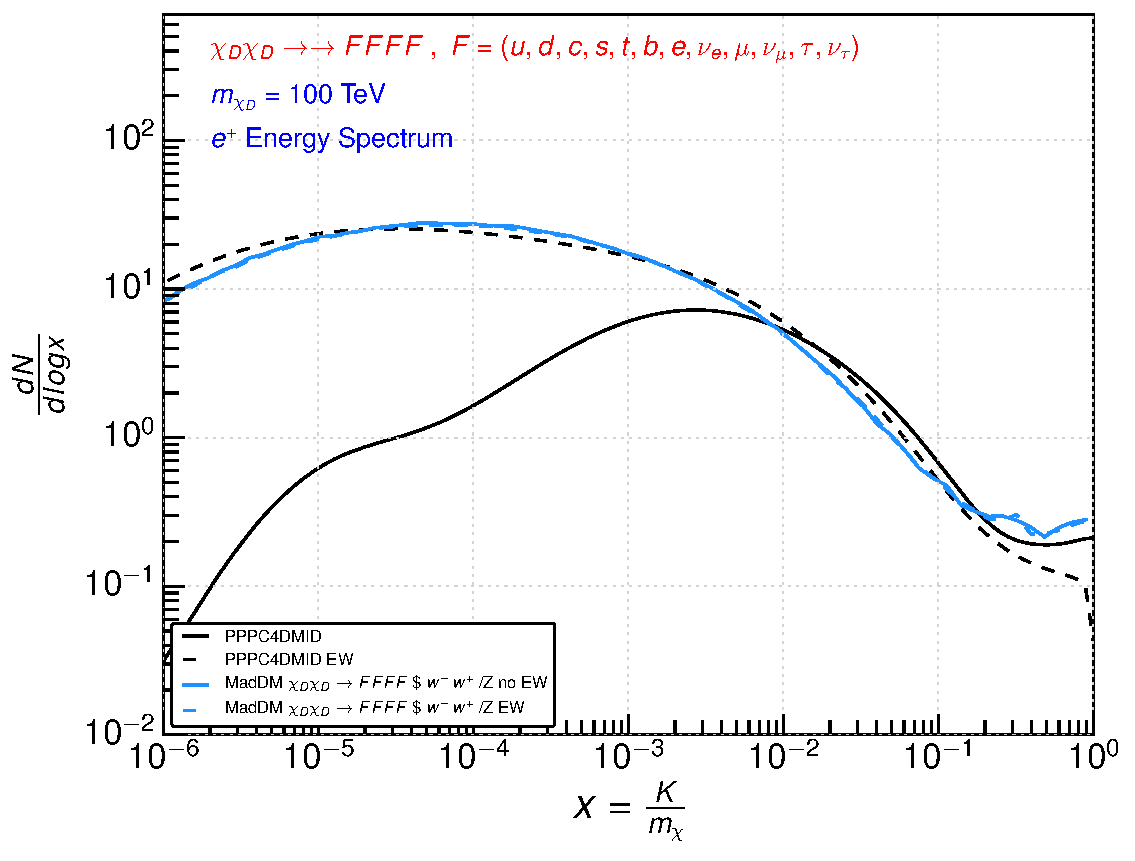
\includegraphics[width=0.49\textwidth]{Fig/xdxd_FFFF_WZ/100_positrons_FFFF_100.pdf}}
\subfigure
{ 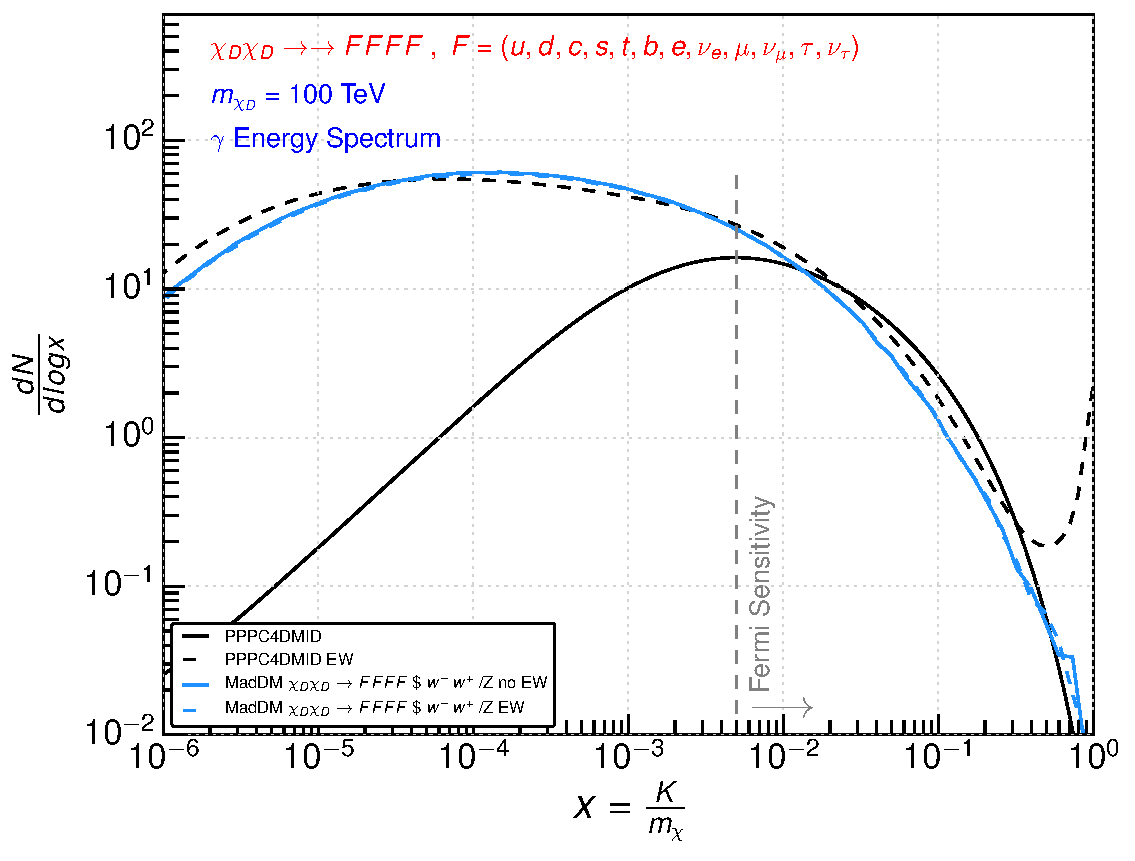
\includegraphics[width=0.49\textwidth]{Fig/xdxd_FFFF_WZ/100_gammas_FFFF_100.pdf}}
\subfigure
{ 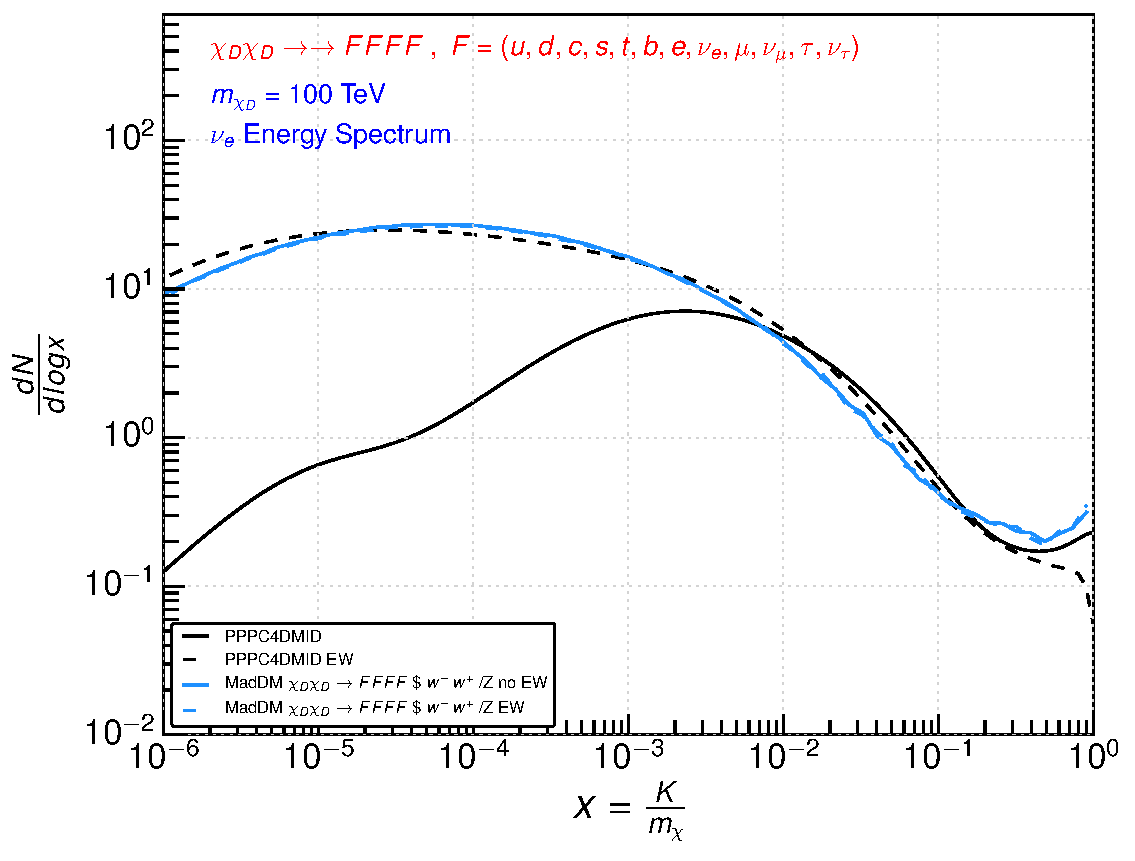
\includegraphics[width=0.49\textwidth]{Fig/xdxd_FFFF_WZ/100_neutrinos_e_FFFF_100.pdf}}
\subfigure
{ 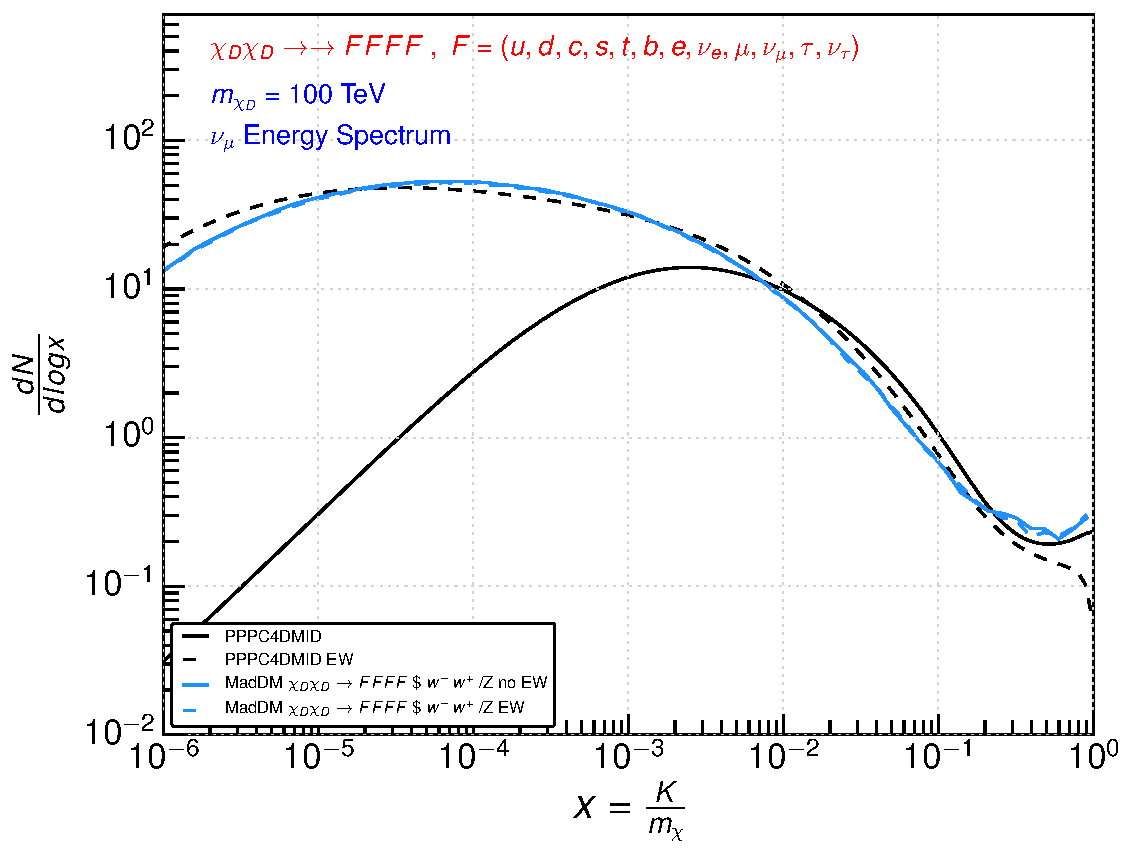
\includegraphics[width=0.49\textwidth]{Fig/xdxd_FFFF_WZ/100_neutrinos_mu_FFFF_100.pdf}}
\subfigure
{ 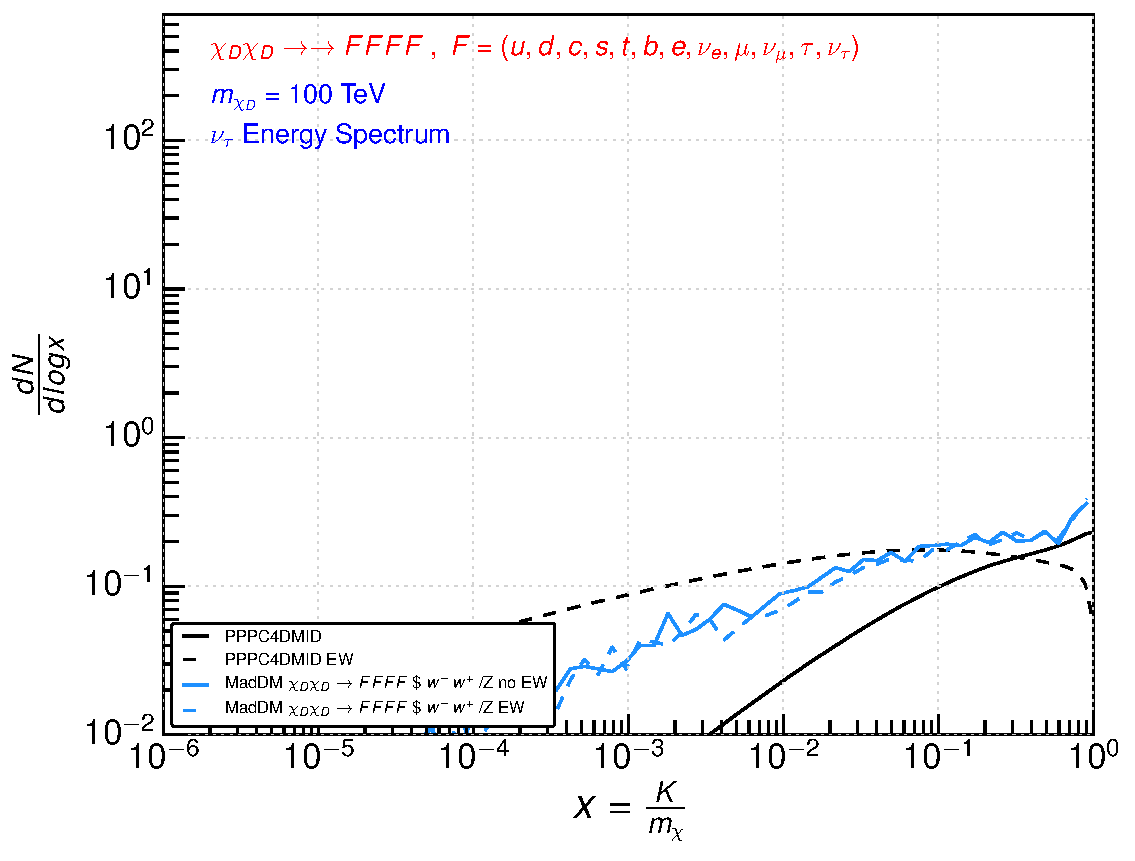
\includegraphics[width=0.49\textwidth]{Fig/xdxd_FFFF_WZ/100_neutrinos_tau_FFFF_100.pdf}}
\caption{Energy Spectra for $m_{\chi_D}$ = 100 TeV for the process $\chi_D \chi_D \rightarrow Y0 \rightarrow FFFF \$w^- w^+ /Z $, for $m_{\chi_D}$ = 1 TeV. The label "EW" and "NoEW" in the MadDM samples mean respectively samples produced with or without the EW corrections in Pythia8.}
\label{woff_100}
\end{figure}

For large $m_{\chi_D}$ masses, the spectra produced with the decays from off-shell $W$ bosons look very similar to the ones from the \PPPCew~. However also note that the electroweak corrections from Pythia 8 don't seem to have any effect at all, i.e. they are not calculated for the 4 fermions. 



\clearpage
\section{MG EW Corrections for $x_d x_d \rightarrow e^- e^+ $}
Process implemented in \MG:
\begin{verbatim}
import model DMsimp_s_spin0_leptons
generate xd xd~ > e- e+
add process xd xd~ > e- e+ z
add process xd xd~ > e+ ve w-
add process xd xd~ > e- ve~ w+
output xdxd_ee_eez_evew
\end{verbatim}
The corresponding Feynman diagrams, for reference, are shown in Fig. \ref{fey}.
\begin{figure}[!h]
	\centering

	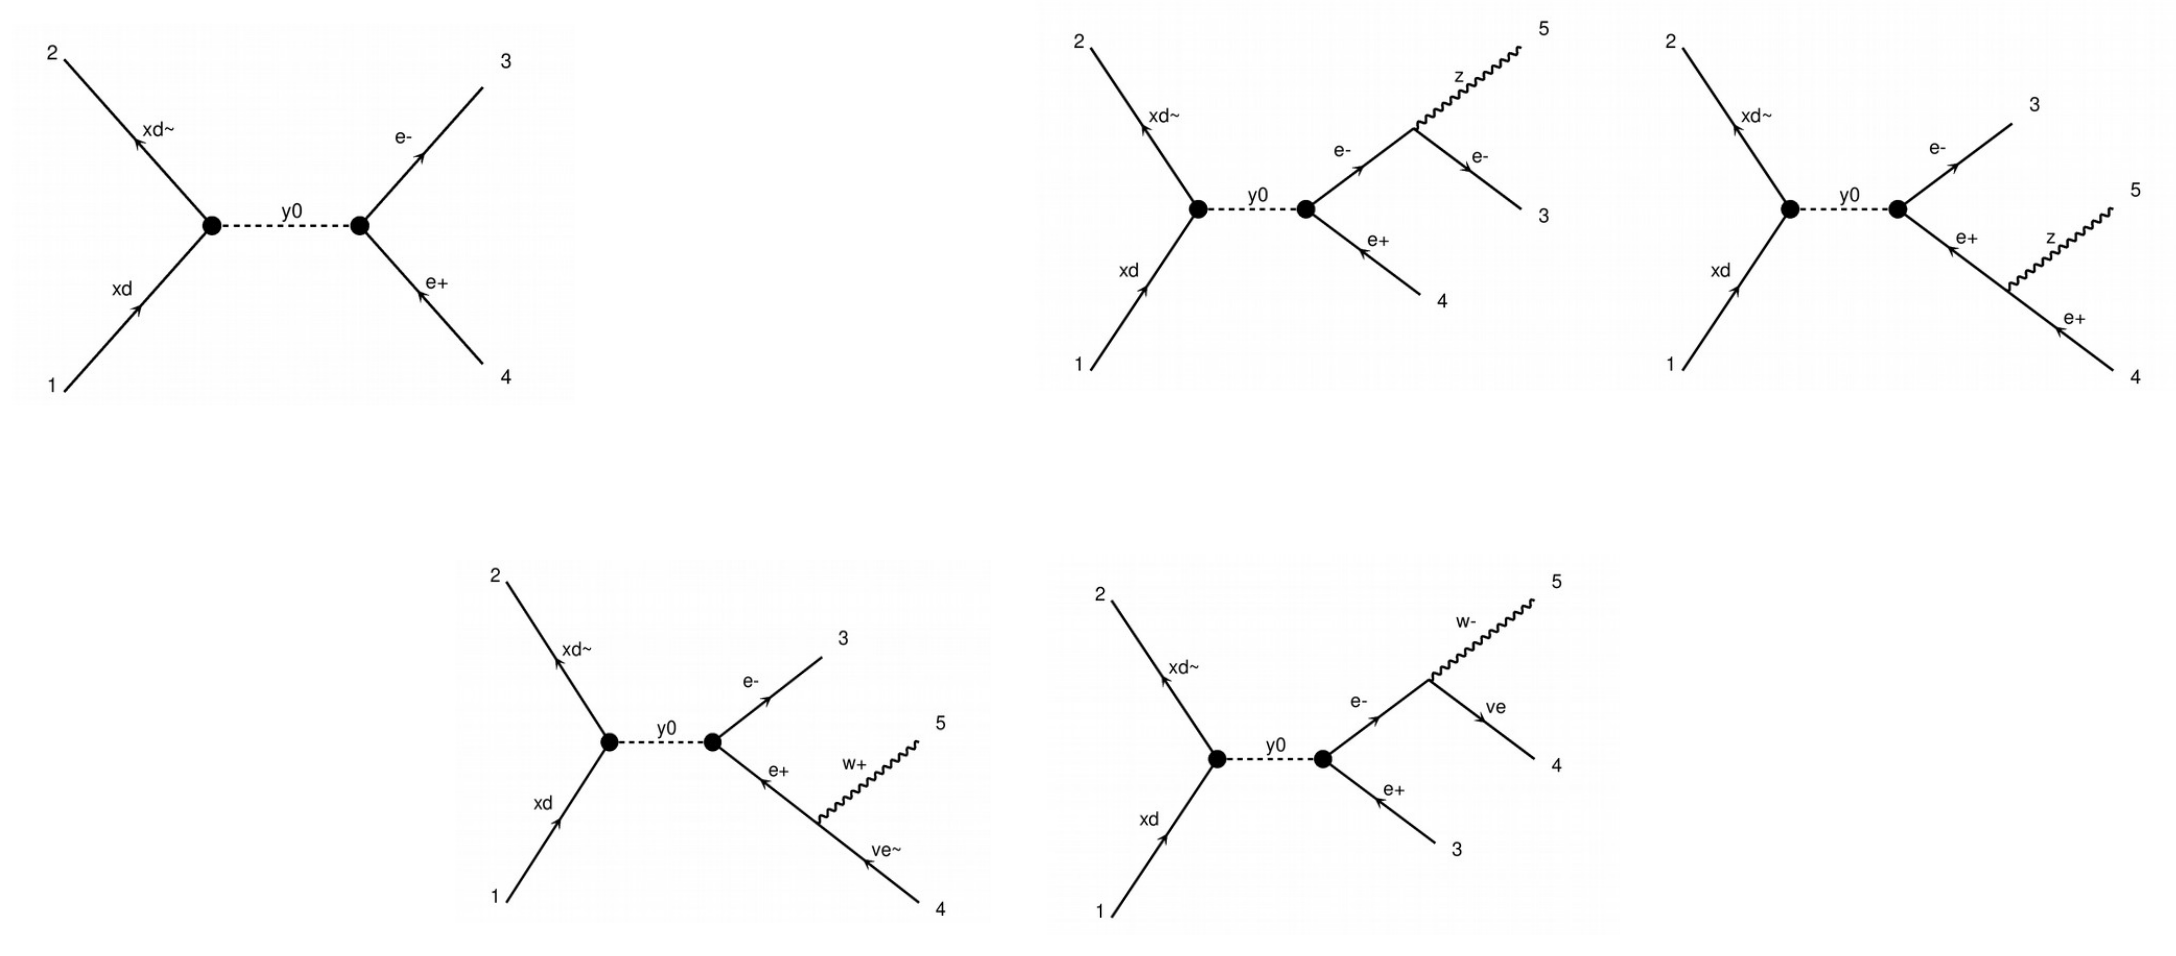
\includegraphics[width=1\textwidth]{Fig/xdxd_ee_eeZ_eveW/Fey.png}}

	\caption{Feynman diagrams.}
	\label{fey}
\end{figure}



\clearpage
\subsection{Kinematic Distributions}
Kinematic distributions of the e,W and Z $p_T$, W and Z boson multiplicities for $m_{x_d}=1$ TeV. Below a certain  $E_{beam}$ threshold, the cross section for the processes are zero except for the "tree-level" $x_d x_d \rightarrow ee$; this was tested with e.g. the process 
\begin{verbatim}
import model DMsimp_s_spin0_leptons
generate xd xd~ > e- e+ z
\end{verbatim}
, which was the reason why I started using higher energy beams than what we usually set (e.g. 1001 or 1010 for $m_{x_d}=1$ ).


\begin{figure}[!h]
	\centering
	\subfigure
	{ 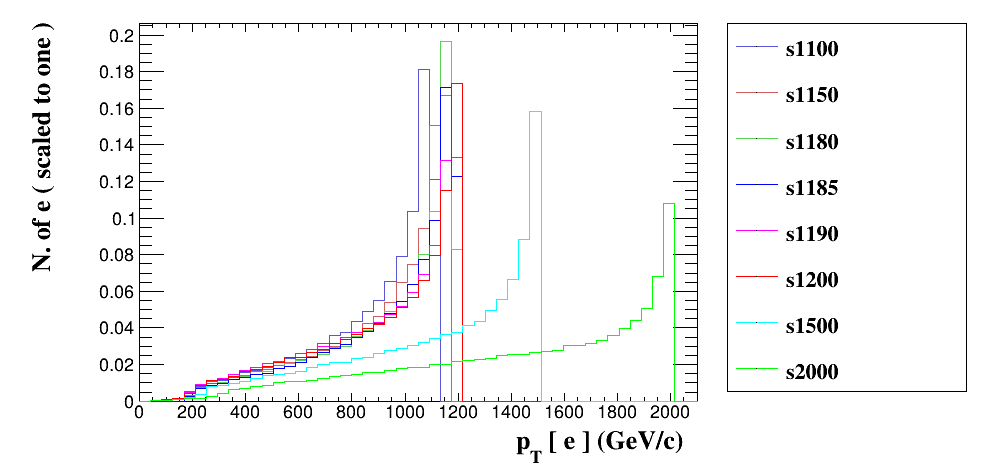
\includegraphics[width=0.49\textwidth]{Fig/xdxd_ee_eeZ_eveW/e_pt.png}}
	\subfigure
{ 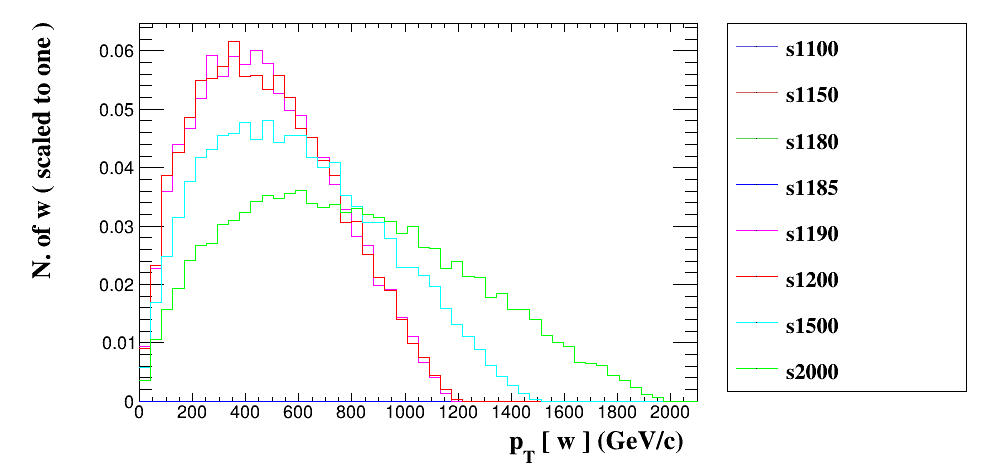
\includegraphics[width=0.49\textwidth]{Fig/xdxd_ee_eeZ_eveW/W_pt.png}}
	\subfigure
{ 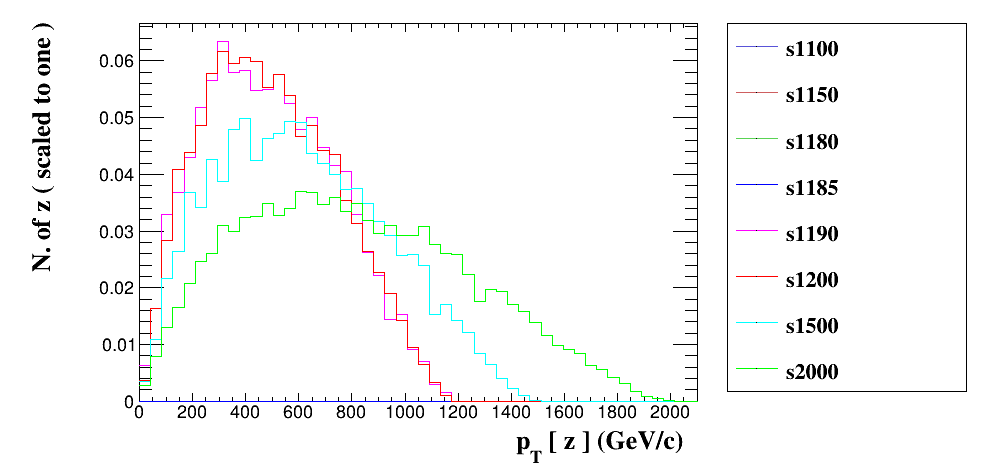
\includegraphics[width=0.49\textwidth]{Fig/xdxd_ee_eeZ_eveW/Z_pt.png}}
	\subfigure
{ 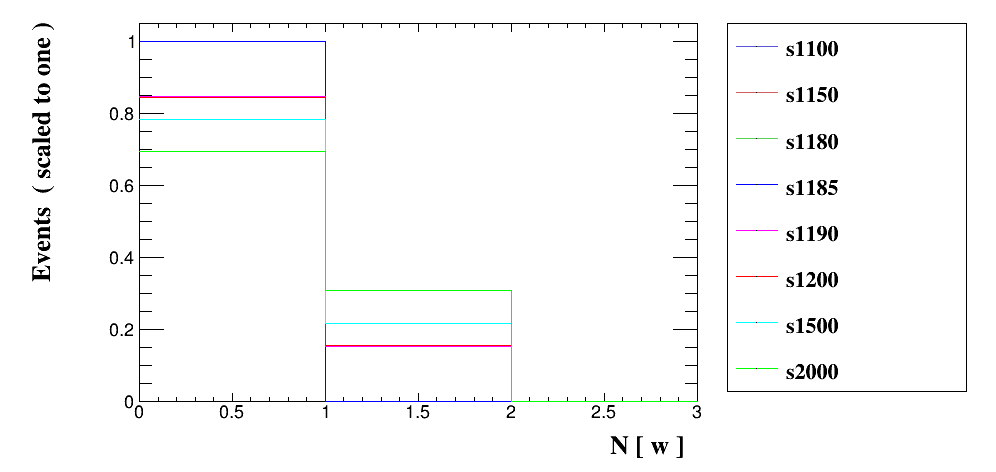
\includegraphics[width=0.49\textwidth]{Fig/xdxd_ee_eeZ_eveW/W_m.png}}
	\subfigure
{ 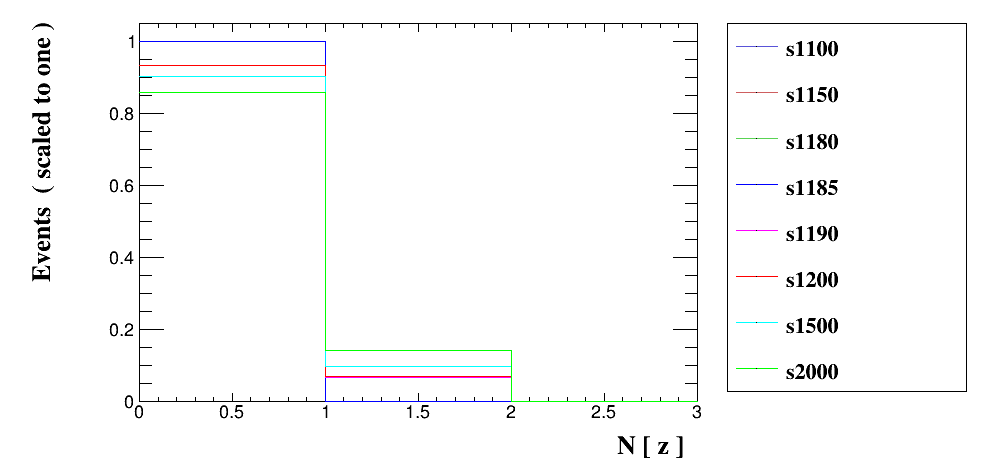
\includegraphics[width=0.49\textwidth]{Fig/xdxd_ee_eeZ_eveW/Z_m.png}}
	
	\caption{Kinematic distributions of the e,W and Z $p_T$, and W and Z multiplicities, for different beams energy ($m_{x_d}=1$ TeV)}.
	\label{woff_100}
\end{figure}

\clearpage
\subsection{Spectra for $m_{xd}=$1 TeV}
\begin{figure}[!h]
	\centering
	\subfigure
	{ 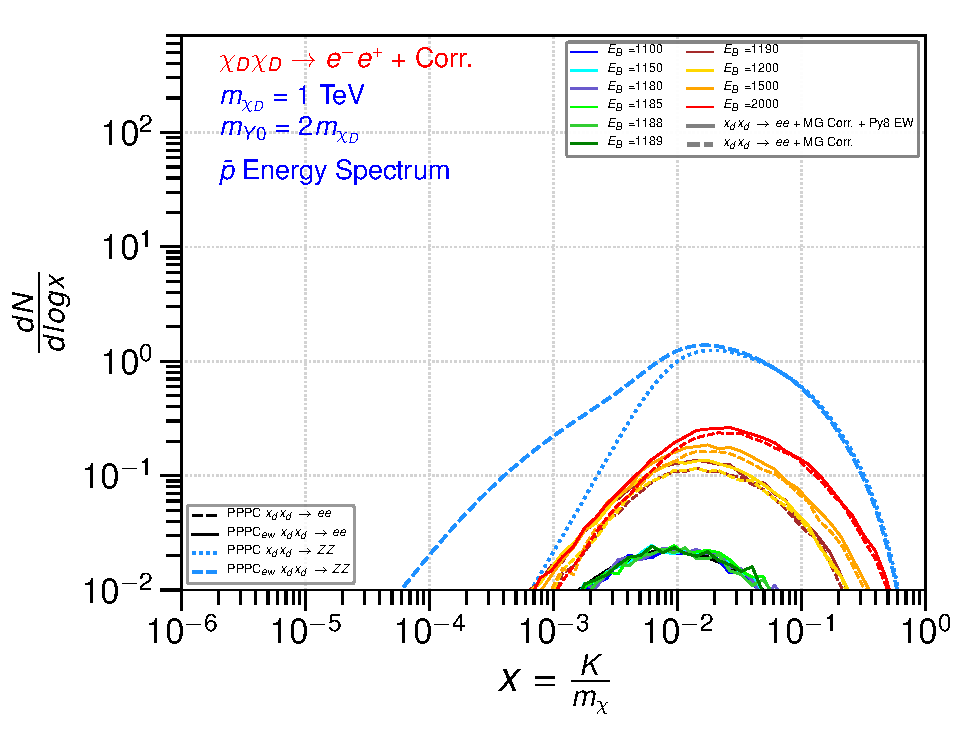
\includegraphics[width=0.49\textwidth]{Fig/xdxd_ee_eeZ_eveW/1_antiprotons_ee_eeZ_eveW_1.pdf}}
	\subfigure
	{ 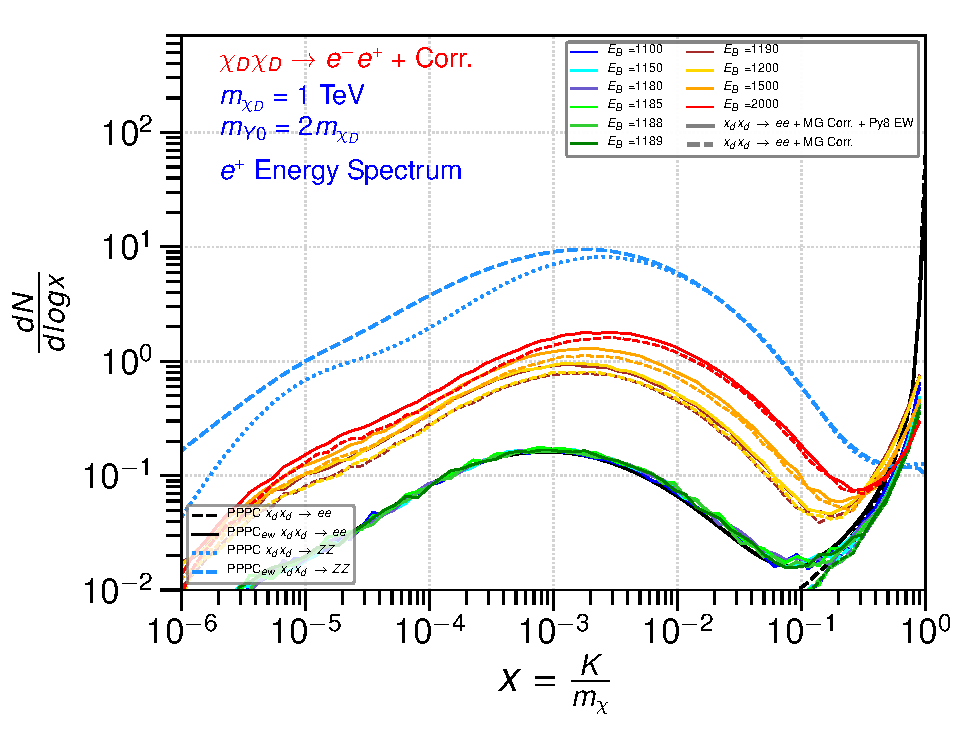
\includegraphics[width=0.49\textwidth]{Fig/xdxd_ee_eeZ_eveW/1_positrons_ee_eeZ_eveW_1.pdf}}
	\subfigure
	{ 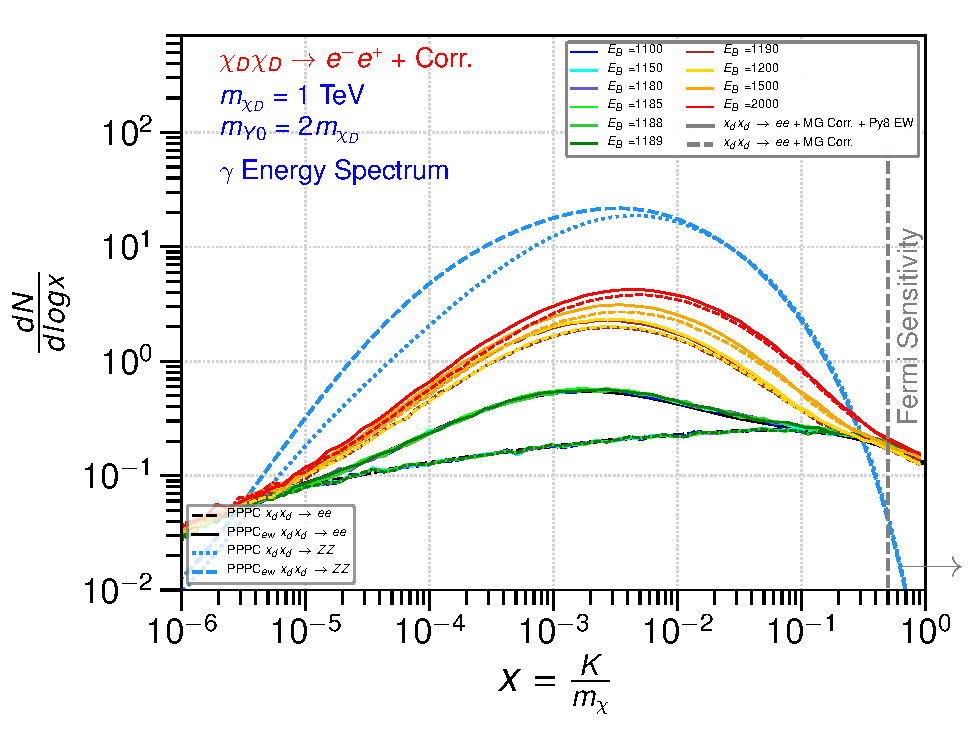
\includegraphics[width=0.49\textwidth]{Fig/xdxd_ee_eeZ_eveW/1_gammas_ee_eeZ_eveW_1.pdf}}
	\subfigure
	{ 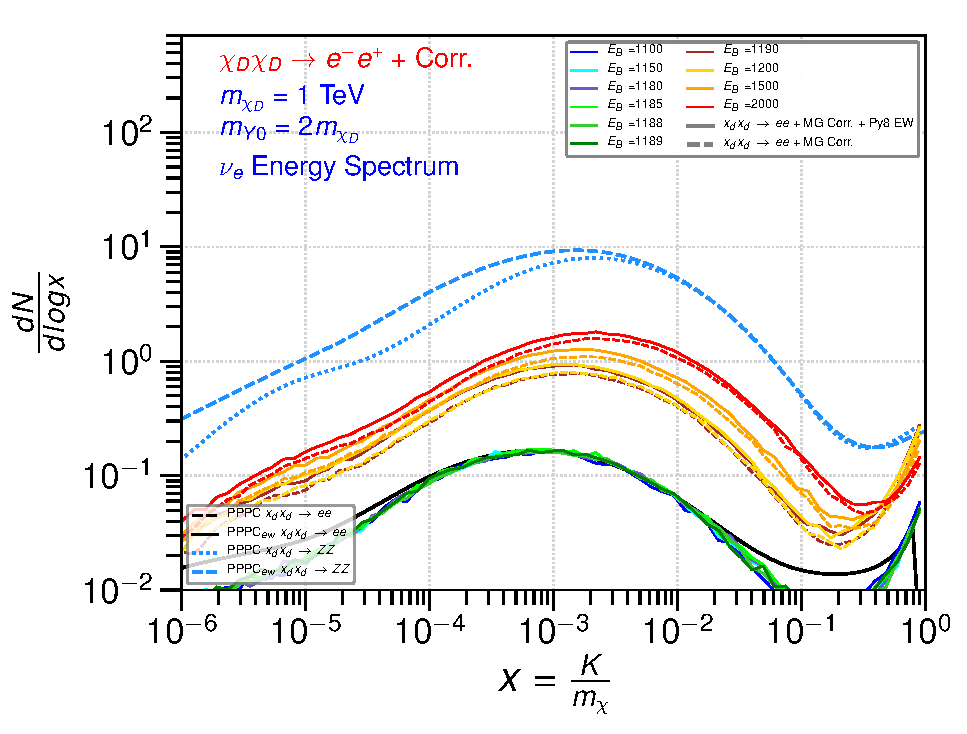
\includegraphics[width=0.49\textwidth]{Fig/xdxd_ee_eeZ_eveW/1_neutrinos_e_ee_eeZ_eveW_1.pdf}}
	\subfigure
	{ \includegraphics[width=0.49\textwidth]{Fig/xdxd_ee_eeZ_eveW/1_neutrinos_mu_ee_eeZ_eveW_1.pdf}}
		\subfigure
	{ \includegraphics[width=0.49\textwidth]{Fig/xdxd_ee_eeZ_eveW/1_neutrinos_tau_ee_eeZ_eveW_1.pdf}}
	\caption{Energy spectra for different beam energies for  $m_/xd=$1 TeV. The process considered is  $x_d x_d \rightarrow e^- e^+ $, with the addition of the EW emission implemented in \MG~. For reference also the spectra for $x_d x_d \rightarrow ZZ $ from the \PPPC and \PPPCew are shown. }.
	\label{spec_eeMGew1}
\end{figure}


\clearpage
\subsection{Spectra for $m_{xd}=$10 TeV}
\begin{figure}[!h]
	\centering
	\subfigure
	{ \includegraphics[width=0.49\textwidth]{Fig/xdxd_ee_eeZ_eveW/10_antiprotons_ee_eeZ_eveW_10.pdf}}
	\subfigure
	{ \includegraphics[width=0.49\textwidth]{Fig/xdxd_ee_eeZ_eveW/10_positrons_ee_eeZ_eveW_10.pdf}}
	\subfigure
	{ \includegraphics[width=0.49\textwidth]{Fig/xdxd_ee_eeZ_eveW/10_gammas_ee_eeZ_eveW_10.pdf}}
	\subfigure
	{ \includegraphics[width=0.49\textwidth]{Fig/xdxd_ee_eeZ_eveW/10_neutrinos_e_ee_eeZ_eveW_10.pdf}}
	\subfigure
	{ \includegraphics[width=0.49\textwidth]{Fig/xdxd_ee_eeZ_eveW/10_neutrinos_mu_ee_eeZ_eveW_10.pdf}}
	\subfigure
	{ \includegraphics[width=0.49\textwidth]{Fig/xdxd_ee_eeZ_eveW/10_neutrinos_tau_ee_eeZ_eveW_10.pdf}}
	\caption{Same as \ref{spec_eeMGew1} for  $m_/xd=$10 TeV}.
	\label{spec_eeMGew10}
\end{figure}


\clearpage
\subsection{Spectra for $m_{xd}=$100 TeV}
\begin{figure}[!h]
	\centering
	\subfigure
	{ \includegraphics[width=0.49\textwidth]{Fig/xdxd_ee_eeZ_eveW/100_antiprotons_ee_eeZ_eveW_100.pdf}}
	\subfigure
	{ \includegraphics[width=0.49\textwidth]{Fig/xdxd_ee_eeZ_eveW/100_positrons_ee_eeZ_eveW_100.pdf}}
	\subfigure
	{ \includegraphics[width=0.49\textwidth]{Fig/xdxd_ee_eeZ_eveW/100_gammas_ee_eeZ_eveW_100.pdf}}
	\subfigure
	{ \includegraphics[width=0.49\textwidth]{Fig/xdxd_ee_eeZ_eveW/100_neutrinos_e_ee_eeZ_eveW_100.pdf}}
	\subfigure
	{ \includegraphics[width=0.49\textwidth]{Fig/xdxd_ee_eeZ_eveW/100_neutrinos_mu_ee_eeZ_eveW_100.pdf}}
	\subfigure
	{ \includegraphics[width=0.49\textwidth]{Fig/xdxd_ee_eeZ_eveW/100_neutrinos_tau_ee_eeZ_eveW_100.pdf}}
	\caption{Same as \ref{spec_eeMGew1} for  $m_/xd=$100 TeV}.
	\label{spec_eeMGew100}
\end{figure}






\clearpage
\section{Cross Sections}
The results of the calculation of various processes cross section are presented. In Fig. \ref{xsec_1TeV} the cross section for different processes are shown. In this case, only the process indicated by the label contributes to the value of the cross section, meaning that e.g. the process $\chi_D \chi_D \rightarrow WW X$ does not include the contribution of the "tree level" process $\chi_D \chi_D \rightarrow WW$. 

\begin{figure}[!b]
	\centering
	\includegraphics[width=0.49\textwidth]{Fig/XSEC/processes_xsec_1_TeV.png}
	\caption{Cross sections for the processes $\chi_D \chi_D \rightarrow WW$ with up to three additional vector bosons $X=W^{\pm} H Z$. Note that only the cross section is relative only to the specific process as indicated by the label is considered (i.e. not the cumulative cross section). The parameters are set to $m_{\chi _D}= 1$ TeV , $m_{Y0}= 2$ TeV, $E_{Beam}=2001$ TeV.}
\label{xsec_1TeV}
\end{figure}
%
Since cross sections depend also on the total energy in the centre-of-mass of the DM annihilation i.e. on the parameter $E_{beam}$ in \MG~, Fig. \ref{xsec_ebeam} shows the cross section values for different energies of the simulated beams.
%
\begin{figure}[!b]
	\centering
	\subfigure
	{ \includegraphics[width=0.32\textwidth]{Fig/XSEC/xsec_Ebeam_1_TeV.png}}
	\subfigure
	{ \includegraphics[width=0.32\textwidth]{Fig/XSEC/xsec_Ebeam_10_TeV.png}}
	\subfigure
	{ \includegraphics[width=0.32\textwidth]{Fig/XSEC/xsec_Ebeam_100_TeV.png}}
	\caption{Cross section of the process $\chi_D \chi_D \rightarrow WW$, for $m_{\chi _D}= 1,10,100$ TeV, for different energies of the beams. The mass of the mediator is set to double the mass of the DM particle.   }
\label{xsec_ebeam}
\end{figure}


\section{Width of the mediator $Y0$ }
When using the automatic computation of the width implemented in \MG~, problems start to arise when the mass of the mediator become large. In particular the width of the particle get to exceed largely the value of its own mass, as it show in Fig. \ref{width}.
Note: this is solved if the parameter $\Lambda$ i.e. the scale of the new physics is set to a value higher than the mass of the DM.
If so, the width of the Y0 becomes stable.
Note that also the cross section scales with $\Lambda$.

\begin{figure}[!h]
	\centering
	\includegraphics[width=0.7\textwidth]{Fig/Widths_check.pdf}

	\caption{Values of the width of the mediatro $Y0$ as calculated by \MG~. A value of $10\%$ of the mediator mass $m_{Y0}$ is shown by the gray line as a comparison.}
	\label{width}
\end{figure}


\clearpage
\section{Unitarity}

As pointed out in e.g. \cite{Kahlhoefer:2015bea}, DM simplified model can face the problem of unitarity violation for specific combinations of the parameters of the model and/or depending on the energy scale. In the cited article, they show that for unitarity to be preserved, the centre-of-mass energy must satisfy:
\begin{equation}
\sqrt{s} < \frac{\pi \ m^2 _{Z'}}{(g^A_{DM})^2 m_{DM})} 
\end{equation}
Using the same formula (which is not exactly applicable to our model), the upper limit on the DM coupling constant $g_{wS}$ can be xtracted as:

\begin{equation}
g_{Sxd} < \sqrt{ \frac{\pi \ m^2 _{Y0}}{ m_{\chi_D} \sqrt{s} }  } 
\end{equation}

The results in Fig.\ref{couplings} show the upper limit values of $g_{Sxd}$ which preserve unitarity, for different DM and mediator masses and beam energies.

\begin{figure}[!b]
	\centering
	\subfigure
	{ \includegraphics[width=0.49\textwidth]{Fig/COUPLINGS/coupling_constant_ul_Mxd_1000.pdf}}
	\subfigure
	{ \includegraphics[width=0.49\textwidth]{Fig/COUPLINGS/coupling_constant_ul_Mxd_10000.pdf}}
	\subfigure
	{ \includegraphics[width=0.49\textwidth]{Fig/COUPLINGS/coupling_constant_ul_Mxd_100000.pdf}}
	\caption{Upper limits on the values of the coupling constant  $g_{Sxd}$  }
	\label{couplings}
\end{figure}

Basically the plots look the same since we always use mxd , my=2*mxd, and Ebeam $\sim$ 2*mxd. So for our standard choices the coupling is fine (set to 1 in the param card).


\clearpage
\section{MG5 Issues}
Sometimes, but not always, I get the following message:
\begin{verbatim}
INFO: Combining Events 
INFO: fail to reach target 10000 
  === Results Summary for run: run_01 tag: tag_1 ===

     Cross-section :   2.711e+06 +- 6.486e+04 pb
     Nb of events :  25
\end{verbatim}
when generating events with extra bosons for \mchi = 100 TeV. The \MG~ version is 2.6.4 .
\clearpage


\section{ {\color{red }  OLD Validation papers arXiv 1009.0224 and 1001.3950 }}
\subsection{Validation Minimal DM Model $x_d x_d \rightarrow \mu^- \mu^+$ + EW arXiv:1001.3950}

\begin{figure}[!h]
	\centering
	\subfigure
	{
		\includegraphics[width=0.48\textwidth]{Fig/Ready/mumu_validation.png} }
	\subfigure
	{
		\includegraphics[width=0.48\textwidth]{Fig/Ready/mumu_validation_basic.png} }
	
	
	\caption{}
	\label{xdxdmumu}
\end{figure}


\subsection{Validation $n_1 n_1 \rightarrow w^- w^+ z$  arXiv:1009.0224}

\begin{figure}[!h]
	\centering

	 \includegraphics[width=0.48\textwidth]{Fig/Ready/kinematic_wwz.pdf}
	\caption{}
	\label{n1n1z}
\end{figure}


\clearpage
\subsection{Validation $n_1 n_1 \rightarrow w^- w^+ \gamma$  arXiv:1009.0224}

\begin{figure}[!h]
	\centering
	\subfigure
	{ \includegraphics[width=0.47\textwidth]{Fig/Ready/Gammas_Validation.pdf} }
	\subfigure
	{ \includegraphics[width=0.47\textwidth]{Fig/Ready/simple_Gammas.pdf} }
	\subfigure
{ \includegraphics[width=0.48\textwidth]{Fig/Ready/Gammas_Validation_nu.pdf} }	
	
	\caption{}
	\label{n1n1a}
\end{figure}

\clearpage
\section{Validation papers arXiv 1009.0224}}
In this section we present the validation of the results for the "Minimal Dark Matter" model introduced in \cite{Ciafaloni:2010ti}. In this DM only has electroweak interactions; we take the case of the parameter space of the MSSM where the DM candidate is a pure Wino-like $\tilde \chi_1 ^0$, and consequently mass degenerate with the lightest chargino $\tilde \chi_1 ^{\pm}$. The results are shown in Fig. \ref{minimal_z}. The plots show the comparison between the results in \cite{Ciafaloni:2010ti} and the results obtained with \maddm~ for the annihilation process $\tilde \chi _1 ^0  \tilde \chi _1 ^0 \rightarrow w^- w^+ z$. The upper plots is obtained for $m_{\tilde \chi_1 ^0}=$ 3 TeV. We see that the \maddm~ results are in good agreement with the theoretical predictions, which are calculated using different approximation methods.  The lower plots compare the \maddm~ distributions with the spectra obtained using Eq.B62b for alternative DM mass of 1 and 10 TeV respectively. Note that Eq.B62b (case of extra Z boson radiation) and  Eq.B62a (case of extra photon radiation) do not produce the correct kinematic boundaries in the low energy boundary of the spectra (according to the authors). Note that the theory predictions for $m_{\tilde \chi_1 ^0}=1,3,10$ TeV were rescaled by multiplying for the arbitrary factors 5,10,3. {\color{blue} I have no idea why but it is the only way to make them to the correct scale.} 
\begin{figure}[!h]
	\centering
	\subfigure
	{ \includegraphics[width=0.55\textwidth]{Fig/Validation_1009/n1n1_wwz_3000.pdf} }
	\subfigure
	{ \includegraphics[width=0.47\textwidth]{Fig/Validation_1009/n1n1_wwz_1000.pdf} }
	\subfigure
    { \includegraphics[width=0.47\textwidth]{Fig/Validation_1009/n1n1_wwz_10000.pdf} }
	
	\caption{Validation of the \maddm~ results with the theoretical prediction from \cite{Ciafaloni:2010ti}, using the "Minimal Dark Matter" model for Wino-like MSSM $\tilde \chi_1 ^0-\tilde \chi_1 ^{\pm}$, for the process  $\tilde \chi _1 ^0  \tilde \chi _1 ^0 \rightarrow w^- w^+ z$. Upper panel: comparison for $m_{\tilde \chi_1 ^0}=$ 3 TeV, the theory predictions are shown in dashed yellow and green lines (line digitized form the original paper, corresponding to two different parametrization used in the analytical calculations) and black dotted (Eq.B62b). In particular, the prediction from the Eq.B62b does not reproduce correctly the low energy tail of the distributions. Lowe panels: comparison for  $m_{\tilde \chi_1 ^0}=$ 1 and 10 TeV.  }
	\label{minimal_z}
\end{figure}

Analogously, the process involving the radiation of one extra photons was validated in Fig. \ref{minimal_z}. Note that due to the cut in the photon energy in the  \textit{run\_card.dat}, the distributions have a sharp edge that does not correspond to actual kinematic boundaries. 

\begin{figure}[!h]
	\centering

 \includegraphics[width=0.55\textwidth]{Fig/Validation_1009/n1n1_wwa.pdf} 

	\caption{Same as Fig. \ref{minimal_z} for the 3-body annihilation process  $\tilde \chi _1 ^0  \tilde \chi _1 ^0 \rightarrow w^- w^+ \gamma$. Note that the edges in the \maddm~ distributions are due to the cut on the photon energy in the \textit{run\_card.dat}.}
	\label{minimal_a}
\end{figure}




\clearpage
\section*{Acknowledgments}
Thanks
%
\bibliographystyle{JHEP}
\bibliography{references}

\end{document}
